% This is samplepaper.tex, a sample chapter demonstrating the
% LLNCS macro package for Springer Computer Science proceedings;
% Version 2.20 of 2017/10/04
%
\documentclass[runningheads]{llncs}
%
\usepackage{graphicx}
% Used for displaying a sample figure. If possible, figure files should
% be included in EPS format.

\usepackage[utf8]{inputenc}
\usepackage[english]{babel}
%\usepackage{amsthm}
\usepackage{amsmath}
\usepackage{amssymb}
\usepackage{float}
\usepackage{hyperref}
\usepackage{booktabs}
\usepackage{caption}
\usepackage{subcaption}
\usepackage[dvipsnames]{xcolor}
\usepackage{bm}
\usepackage[makeroom]{cancel}

\usepackage[ruled,vlined]{algorithm2e}
%\newcommand\mycommfont[1]{\footnotesize\ttfamily\textcolor{blue}{#1}}
%\SetCommentSty{mycommfont}
\SetKwComment{Comment}{$\triangleright$\ }{}

\usepackage[%
square,        % for square brackets
comma,         % use commas as separators
%  numbers,       % for numerical citations;
%  sort,          % orders multiple citations into the sequence in which they appear in the list of references;
sort&compress, % as sort but in addition multiple numerical citations
% are compressed if possible (as 3-6, 15);
]{natbib}
% In the bibliography, references have to be formatted as 1., 2., ... not [1], [2], ...
\renewcommand{\bibnumfmt}[1]{#1.}

\renewcommand{\bibsection}{\section*{References}} % requried for natbib to have "References" printed and as section*, not chapter*
% Use natbib compatbile splncsnat style.
% It does provide all features of splncs03, but is developed in a clean way.
% Source: http://phaseportrait.blogspot.de/2011/02/natbib-compatible-bibtex-style-bst-file.html
\bibliographystyle{splncsnat}

\usepackage{todonotes}
\newcommand{\oam}[1]{\todo[inline,color=orange!40]{{\textbf{OM:}~}#1}}
\newcommand{\el}[1]{\todo[inline,color=green!40]{{\textbf{EL:}~}#1}}



%%%%%%%%%%%%%%%%%%%%%%%%%%%%
% Paper dependent stuff    %
%%%%%%%%%%%%%%%%%%%%%%%%%%%%

\newcommand{\Tau}{T}

\newcommand{\hlrb}[1]{\bm{\textcolor{Red}{#1}}}
\newcommand{\hlbb}[1]{\bm{\textcolor{Blue}{#1}}}
\newcommand{\hlgb}[1]{\bm{\textcolor{Green}{#1}}}

\newcommand{\OPD}{\texttt{OPD}}

%%%%%%%%%%%%%%%%%%%%%%%%%%%%
% Aesthetics               %
% over-underline, hat, bold%
%%%%%%%%%%%%%%%%%%%%%%%%%%%%

\newcommand{\eps}{\varepsilon}
\newcommand{\vareps}{\varepsilon}
\renewcommand{\epsilon}{\varepsilon}
%\renewcommand{\hat}{\widehat}
\renewcommand{\tilde}{\widetilde}
\renewcommand{\bar}{\overline}

\newcommand*{\MyDef}{\mathrm{\tiny def}}
\newcommand*{\eqdefU}{\ensuremath{\mathop{\overset{\MyDef}{=}}}}% Unscaled version
% \newcommand*{\eqdef}{\mathop{\overset{\MyDef}{\resizebox{\widthof{\eqdefU}}{\heightof{=}}{=}}}}
\newcommand{\eqdef}{\stackrel{def}{=}}


\def\:#1{\protect \ifmmode {\mathbf{#1}} \else {\textbf{#1}} \fi}
\newcommand{\CommaBin}{\mathbin{\raisebox{0.5ex}{,}}}

\newcommand{\wt}[1]{\widetilde{#1}}
\newcommand{\wh}[1]{\widehat{#1}}
\newcommand{\wo}[1]{\overline{#1}}
\newcommand{\wb}[1]{\overline{#1}}

% bf and bm missing due to conflict!!
\newcommand{\bsym}[1]{\mathbf{#1}}
\newcommand{\bzero}{\mathbf{0}}
\newcommand{\ba}{\mathbf{a}}
\newcommand{\bb}{\mathbf{b}}
\newcommand{\bc}{\mathbf{c}}
\newcommand{\bd}{\mathbf{d}}
\newcommand{\be}{\mathbf{e}}
\newcommand{\bg}{\mathbf{g}}
\newcommand{\bh}{\mathbf{h}}
\newcommand{\bi}{\mathbf{i}}
\newcommand{\bj}{\mathbf{j}}
\newcommand{\bk}{\mathbf{k}}
\newcommand{\bl}{\mathbf{l}}
\newcommand{\bn}{\mathbf{n}}
\newcommand{\bo}{\mathbf{o}}
\newcommand{\bp}{\mathbf{p}}
\newcommand{\bq}{\mathbf{q}}
\newcommand{\br}{\mathbf{r}}
\newcommand{\bs}{\mathbf{s}}
\newcommand{\bt}{\mathbf{t}}
\newcommand{\bu}{\mathbf{u}}
\newcommand{\bv}{\mathbf{v}}
\newcommand{\bw}{\mathbf{w}}
\newcommand{\bx}{\mathbf{x}}
\newcommand{\by}{\mathbf{y}}
\newcommand{\bz}{\mathbf{z}}

\newcommand{\bA}{\mathbf{A}}
\newcommand{\bB}{\mathbf{B}}
\newcommand{\bC}{\mathbf{C}}
\newcommand{\bD}{\mathbf{D}}
\newcommand{\bE}{\mathbf{E}}
\newcommand{\bF}{\mathbf{F}}
\newcommand{\bG}{\mathbf{G}}
\newcommand{\bH}{\mathbf{H}}
\newcommand{\bI}{\mathbf{I}}
\newcommand{\bJ}{\mathbf{J}}
\newcommand{\bK}{\mathbf{K}}
\newcommand{\bL}{\mathbf{L}}
\newcommand{\bM}{\mathbf{M}}
\newcommand{\bN}{\mathbf{N}}
\newcommand{\bO}{\mathbf{O}}
\newcommand{\bP}{\mathbf{P}}
\newcommand{\bQ}{\mathbf{Q}}
\newcommand{\bR}{\mathbf{R}}
\newcommand{\bS}{\mathbf{S}}
\newcommand{\bT}{\mathbf{T}}
\newcommand{\bU}{\mathbf{U}}
\newcommand{\bV}{\mathbf{V}}
\newcommand{\bW}{\mathbf{W}}
\newcommand{\bX}{\mathbf{X}}
\newcommand{\bY}{\mathbf{Y}}
\newcommand{\bZ}{\mathbf{Z}}

% calligraphic
\newcommand{\cf}{\mathcal{f}}
\newcommand{\cA}{\mathcal{A}}
\newcommand{\cB}{\mathcal{B}}
\newcommand{\cC}{\mathcal{C}}
\newcommand{\cD}{\mathcal{D}}
\newcommand{\cE}{\mathcal{E}}
\newcommand{\cF}{\mathcal{F}}
\newcommand{\cG}{\mathcal{G}}
\newcommand{\cH}{\mathcal{H}}
\newcommand{\cI}{\mathcal{I}}
\newcommand{\cJ}{\mathcal{J}}
\newcommand{\cK}{\mathcal{K}}
\newcommand{\cL}{\mathcal{L}}
\newcommand{\cM}{\mathcal{M}}
\newcommand{\cN}{\mathcal{N}}
\newcommand{\cO}{\mathcal{O}}
\newcommand{\cP}{\mathcal{P}}
\newcommand{\cQ}{\mathcal{Q}}
\newcommand{\cR}{\mathcal{R}}
\newcommand{\cS}{\mathcal{S}}
\newcommand{\cT}{\mathcal{T}}
\newcommand{\cU}{\mathcal{U}}
\newcommand{\cV}{\mathcal{V}}
\newcommand{\cW}{\mathcal{W}}
\newcommand{\cX}{\mathcal{X}}
\newcommand{\cY}{\mathcal{Y}}
\newcommand{\cZ}{\mathcal{Z}}

%%%%%%%%%%%%%%%%%%%%%%%%%%%%
% Math jargon              %
%%%%%%%%%%%%%%%%%%%%%%%%%%%%
\newcommand{\wrt}{w.r.t.\xspace}
\newcommand{\defeq}{\stackrel{\mathclap{\normalfont\mbox{\tiny def}}}{=}}
\newcommand{\maxund}[1]{\max\limits_{#1}}
\newcommand{\supund}[1]{\text{sup}\limits_{#1}}
\newcommand{\minund}[1]{\min\limits_{#1}}
\renewcommand{\epsilon}{\varepsilon}
\newcommand{\bigotime}{\mathcal{O}}


\DeclareMathOperator*{\argmin}{arg\,min} 
\DeclareMathOperator*{\argmax}{arg\,max} 
\DeclareMathOperator*{\cupdot}{\mathbin{\mathaccent\cdot\cup}}

%%%%%%%%%%%%%%%%%%%%%%%%%%%%
% Matrix operators         %
%%%%%%%%%%%%%%%%%%%%%%%%%%%%
\newcommand{\transpose}{^\mathsf{\scriptscriptstyle T}}
\newcommand{\transp}{\mathsf{\scriptscriptstyle T}}

%%%%%%%%%%%%%%%%%%%%%%%%%%%%
% Statistic operators      %
%%%%%%%%%%%%%%%%%%%%%%%%%%%%
\newcommand{\probability}[1]{\mathbb{P}\left(#1\right)}
\newcommand{\probdist}{Pr}
\DeclareMathOperator*{\expectedvalue}{\mathbb{E}}
\DeclareMathOperator*{\variance}{\text{Var}}
\newcommand{\expectedvalueover}[1]{\expectedvalue\limits_{#1}}
\newcommand{\condbar}{\;\middle|\;}
\newcommand{\gaussdistr}{\mathcal{N}}
\newcommand{\uniformdistr}{\mathcal{U}}
\newcommand{\bernoullidist}{\mathcal{B}}

%%%%%%%%%%%%%%%%%%%%%%%%%%%%
% Algebraic Sets           %
%%%%%%%%%%%%%%%%%%%%%%%%%%%%
\newcommand{\Real}{\mathbb{R}}
\newcommand{\Natural}{\mathbb{N}}
\newcommand{\statespace}{\mathcal{X}}
\newcommand{\funcspace}{\mathcal{F}}
\newcommand{\dynaspace}{\mathcal{T}}

%
%\newtheorem{theorem}{Theorem}
%\newtheorem{definition}{Definition}
%\newtheorem{lemma}{Lemma}
%\providecommand*\lemmaautorefname{Lemma}
%\newtheorem{proposition}{Proposition}
%\providecommand*\propositionautorefname{Proposition}
%\newtheorem{remark}{Remark}
%\newtheorem{property}{Property}
%\newtheorem{assumption}{Assumption}
%\providecommand*\assumptionautorefname{Assumption}
%\newtheorem{conjecture}{Conjecture}
\providecommand*\algorithmautorefname{Algorithm}

\addto\extrasenglish{  
	\def\algorithmautorefname{Algorithm}  
}
%
%\newtheorem*{definition*}{Definition}
%\newtheorem*{theorem*}{Theorem}
%\newtheorem*{proposition*}{Proposition}
%\newtheorem*{remark*}{Remark}
% If you use the hyperref package, please uncomment the following line
% to display URLs in blue roman font according to Springer's eBook style:
 \renewcommand\UrlFont{\color{blue}\rmfamily}

\begin{document}


\title{Graph-Based Optimistic Planning}
%
%\titlerunning{Abbreviated paper title}
% If the paper title is too long for the running head, you can set
% an abbreviated paper title here
%
\author{Edouard Leurent\inst{1,2}\and Odalric-Ambrym Maillard\inst{1}}
%
\authorrunning{E. Leurent and O-A. Maillard}
% First names are abbreviated in the running head.
% If there are more than two authors, 'et al.' is used.
%
\institute{SequeL project, INRIA Lille - Nord Europe, France\\
\email{$\{$edouard.leurent,odalric.maillard$\}$@inria.fr}\and
Renault Group, France
%\\
%\email{edouard.leurent@renault.com}
}
%
\maketitle              % typeset the header of the contribution
%
\begin{abstract}
	We consider the problem of planning in a Markov Decision Process (MDP) with a generative model and limited computational budget. Despite the underlying MDP transitions having a graph structure, the popular \emph{tree-based} planning algorithms such as \texttt{UCT} rely on a tree structure to represent their value estimates. That is, they either ignore the states crossed along a trajectory, or they do not identify with each other two similar states met at different places in the tree. In this work, we explore taking into account state similarity by proposing a \emph{graph-based} planning algorithm. For the sake of analysis and explicit comparison with tree-based planners, we first study how to augment such tree-based planners with a \emph{state aggregation} operator, in the simple case of deterministic systems. We provide a regret bound that depends on a novel problem-dependent measure of difficulty. This measure improves on the previous one in MDPs where the trajectories overlap, and recovers it otherwise. Then, we reformulate our algorithm in the more natural graphical setting where the state aggregation is implicit, and show that it can be adapted to planning with stochastic systems. Finally, numerical simulations illustrate the benefits of our approach.
	
	\keywords{Planning  \and Tree-search \and Online learning.} % TODO
\end{abstract}
%
%
%

\section{Introduction}

In a \emph{Markov Decision Process} (MDP), an agent observes its current state $s$ from a state space $S$ and picks an action $a$ from an action space $A$, before transitioning to a next state $s'$ drawn from a transition kernel $\probability{s'\condbar s,a}$ and receiving a bounded reward $r\in[0, 1]$ drawn from a reward kernel $\probability{r \condbar s, a}$. The transition kernel can be seen as a \emph{graph}, where the nodes correspond to states $s\in S$, and the edges to transition probabilities between two states. The goal of the agent is act so as to maximise in expectation its cumulative discounted rewards $\sum_{t=0}^\infty \gamma^t r(s_t, a_t)$, where $\gamma\in(0, 1)$ is a discount factor. This amounts to choosing at each step the action that maximises the state-action value function $Q$ defined as:
\begin{align*}
Q(s, a) &= \max_\pi  \expectedvalue_\tau \left[\sum_{t=0}^\infty \gamma^t r(s_t, a_t)\condbar s_0 = s, a_0 = a\right]
\end{align*}
where $\pi$ is a policy mapping states to actions and $\tau = (s_0, a_0, \dots)$ is a trajectory generated by following $\pi$. In an \emph{online planning} setting, the underlying MDP is \emph{unknown} to the agent which only has access to a \emph{generative model} that provides samples $s'$ of $\probability{s' \condbar s, a}$ when queried. Then, under computational constraints known as \emph{fixed-budget}, the agent is allowed to generate a limited number $n$ of trajectories starting from its current state before recommending a good action $a_n$ to take next.
The quality of that action is assessed in terms of the \emph{simple regret}
\begin{align}
	r_n \eqdef V(s) - Q(s, {a}_n), \; \mbox{where} \; V(s) \eqdef  \max_a Q(s, a).
\end{align}

Tree-based planning algorithms. They date back to the work of \citet{Kearns02SS}, who proposed a uniform sampling approach for planning in MDPs, called \texttt{Sparse} \texttt{Sampling}. This uniform exploration strategy was further analysed with the \texttt{BRUE} algorithm
\citep{Feldman14BRUE} providing an enhanced value estimation procedure. Another family of algorithms rely on the principle of \emph{Optimism in the Face of Uncertainty} \citep[surveyed by][]{SurveyRemiMCTS}, inspired from the Multi-Armed Bandit problem. This principle was first used in the context of planning in the \texttt{CrazyStone} software \citep{Coulom2006} for computer Go. It was later analysed as the \texttt{UCT} algorithm \citep{Kocsis06UCT}, but was shown by \citet{Coquelin2007} to have a doubly-exponential complexity in the worst case. The {Optimistic Planning for Deterministic Systems} (\texttt{OPD}) algorithm introduced by \citet{hren2008optimistic} was the first to provide a polynomial regret bound, but was limited to sytems with deterministic rewards and dynamics. It was then extended to the {open-loop} setting to handle stochastic rewards \citep{bubeck2010open,leurent2019practical}.
MDP with known parameters \citep{busoniu2012optimistic}.
For MDPs with stochastic and unknown transitions, polynomial sample complexities have been obtained for StOP \citep{STOP14}, TrailBlazer \citep{TrailBlazer16} and SmoothCruiser \citep{SmoothCruiser19} but the three algorithms suffer from numerical inefficiency.



\emph{All} the planning algorithms mentioned so far have one thing in common: they \emph{do not merge information across states}.
% A node is identified with the sequence of $h$ states and actions that leads to it. It leads to a very simple update: after each trajectory, one only needs to update the confidence bounds, $U_h(s_h,a_h)$ and $L_h(s_h,a_h)$, of the visited action-state pairs, see Algorithm~\ref{alg:OptimisticVItraj}. %The complexity of this value iteration is only of order $O(KBH)$ in time and $O(H)$ in space (since we only need to keep the last trajectory).
% Another option is to merge information for the same states and a fixed depth. But in this case the search tree becomes a \emph{graph} and after each trajectory we need to re-compute the values $U_h(s_h,a_h)$ for all stored state action pairs $(s_h,a_h)$ at each depth, see
% %we thus need to update  perform a complete optimistic value iteration to update the confidence bounds, see
% Algorithm~\ref{alg:OptimisticVIcompl}.
% %The complexity of this algorithm is of order $O(KBH)$ in time and $O(H)$.


If two trajectories $\tau_1$, $\tau_2$ lead to the same state $s$, the latter is actually modelled as two different states $s^1$ and $s^2$ and the information is not shared between the two trajectories. A local update can require to propagate information through the entire tree.

\paragraph{Contributions}

\paragraph{Outline}


\section{Graph-Based Planning for Deterministic Systems}

We consider the simple setting of MDPs with deterministic dynamics and rewards.
We start by giving some background on the interplay of data structures and optimistic planning algorithms.

\subsection{Data structures}

In this work, we will be comparing two data structures for planning in an MDP: the tree, and the (directed) graph. In order to differentiate them, we use Roman symbols when referring to the trees, e.g. $T, U, L, B$ and calligraphic symbols when referring to the graphs, e.g. $\cG, \cU, \cL, \cB$.

\paragraph{In a tree,} a node of depth $h$ represents a sequence of actions $a\in A^h$. The \textit{root} of the tree corresponds to the empty action sequence, and hence to the initial state $s_0\in S$. At iteration $n$, we denote the current tree as $\Tau_n$. Borrowing notations from topology, we denote its set of internal nodes as $\mathring{\Tau}_n$ and its set of \textit{leaves} as $\overline{\Tau}_n$. Note that since the MDP is deterministic, a sequence of action $a$ is associated with its terminal state denoted $s(a)$, but this association is not one-to-one: several sequences of action can lead to the same state, and the latter will be represented several times in the tree. Thus, we denote $N_n(a)$ the set of \emph{neighbours} of a sequence of action $a\in A^h$, that lead to the same state:  $N_n(a) = \{a'\in\Tau_n: s(a)=s(a')\}.$

\begin{figure}[H]
	\centering
	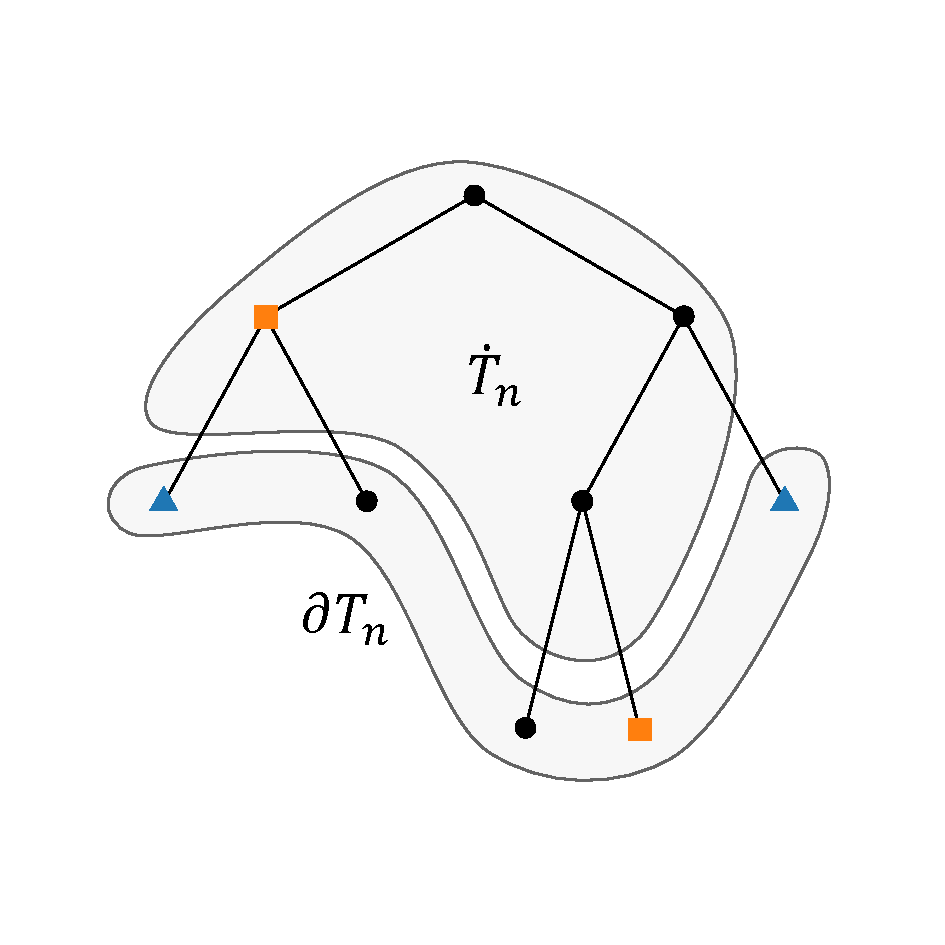
\includegraphics[trim={1.8cm 1.2cm 1.9cm 1.2cm}, clip,width=0.44\linewidth]{img/tree_1}
	\hfill
	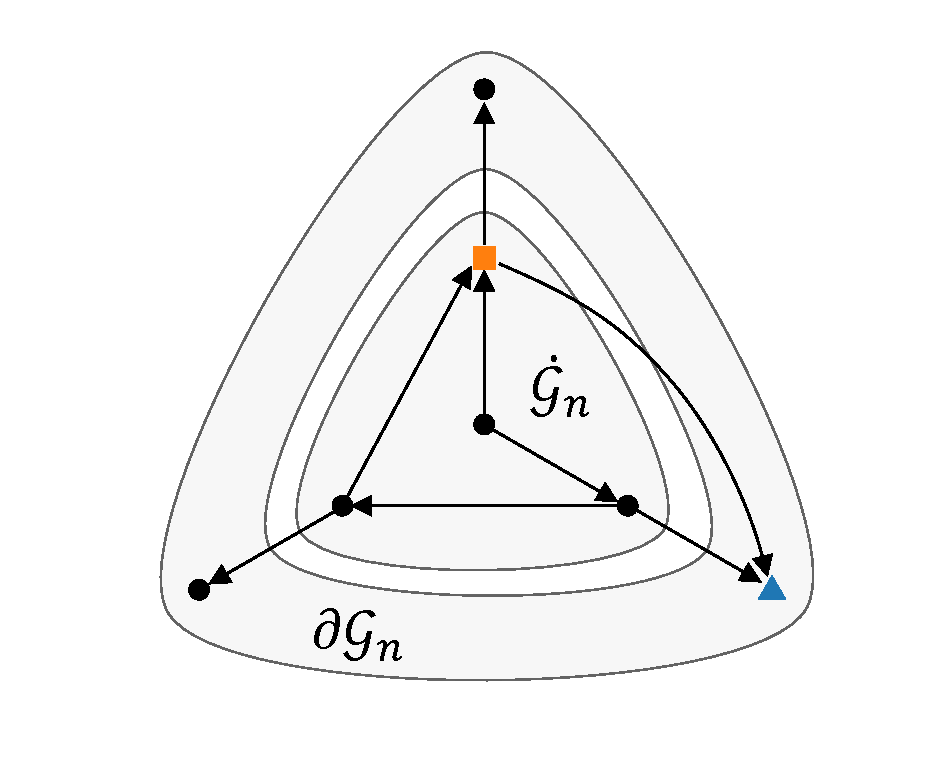
\includegraphics[trim={1.8cm 1.2cm 1.9cm 0.9cm}, clip,width=0.44\linewidth]{img/graph_1}
	\caption{Depiction of the tree $\Tau_n$ (left) and the graph $\cG_n$ (right) built with the same observed transitions. In the tree, two nodes of the same colour lead to the same state.}
\end{figure}

\paragraph{In a graph,} the nodes represent states $s\in S$, and the edges represent transitions between states. The \textit{source} of the tree corresponds to the initial state $s_0$. At iteration $n$, we denote the current graph as $\cG_n$, its set of internal nodes as $\mathring{\cG}_n$ and its set of \textit{sinks} as $\overline{\cG}_n$.

Both structures are built iteratively from a single starting node, by selecting an exterior node (leaf or sink) to \emph{expand}. The expansion of a node $a$ or $s$ refers to calling the generative model to sample the reward $r$ and next state $s'$ for each action $a\in A$, and adding child nodes to the data structure. In a tree, the expansion of a node $a\in A^h$ always lead to the creation of new leaf nodes that represent the suffix sequence of action $ab\in A^{h+1},\, b\in A$. In contrast, in a graph the next state $s'$ reached from $s,a$ might already be present in $\cG_n$, in which case we add the edge between $s$ and $s'$ without creating a new node.

These data structures can be used to store information about the MDP, such as its rewards $r(s, a)$, so that 


\subsection{Planning algorithms}

A planning algorithm is typically composed of two main rules:
\begin{enumerate}
	\item A \emph{sampling rule}, that selects a promising exterior node (leaf or sink) to expand at each iteration $n$.
	\item A \emph{recommendation rule}, that recommends a first good action to take at the last iteration $n$.
\end{enumerate}
The pseudo-code of such a planning algorithm is given in \autoref{alg:generic}.
\begin{algorithm}
	\caption{A generic planning algorithm}
	\label{alg:generic}
	\DontPrintSemicolon
	\For{each iteration $n$}{
		Select the node $\hat{a}_n$ (or $\hat{s_n}$) to expand according to the sampling rule.\;
		\For(\Comment*[f]{Node expansion}){action $a\in A$}{
			Simulate the transition $r, s' \sim \probability{r, s' \condbar s, a}$ from the generative model.\;
			Insert the observed transition to the data structure accordingly.
		}
	}
	\Return the recommended action $a_{n}$ according to the recommendation rule.\;
\end{algorithm}

But how to choose the sampling and recommendation rule? \todo{Etoffer}

\subsection{Optimistic planning}

The principle of \emph{Optimism in the Face of Uncertainty} consists in exploring the option that maximises an upper-bound of the true objective. It has been applied in the context of planning by forming bounds on the value function $V$ (or $Q$).

\begin{definition}[Value bounds]
\paragraph{On trees.} We denote by $L:\Tau_n \rightarrow \Real$ and  $U:\Tau_n \rightarrow \Real$ a lower-bound and upper-bound for the state-value $V(s(a))$ defined on the tree $\Tau_n$, such that
\begin{equation*}
    \forall a\in\Tau_n, \qquad L(a) \leq V(s(a)) \leq U(a).
\end{equation*}

\paragraph{On graphs.} Likewise, we denote by $\cL:\cG_n \rightarrow \Real$ and  $\cU:\cG_n \rightarrow \Real$ a lower-bound and upper-bound for the state-value $V(s(a))$ defined on the graph $\cG_n$, such that
\begin{equation*}
\forall s\in\cG_n, \qquad \cL(s) \leq V(s) \leq \cU(s).
\end{equation*}
\end{definition}

Following the OFU principle, at iteration $n$ we leverage available information to design an upper-bound $U_n$ on $V$, which should be as tight as possible. Then, the sampling rule will select an exterior node by starting from the root / source and following an optimistic strategy of always selecting the action which maximises $U_n$, until reaching an optimistic leaf / sink to expand.

For instance, since we assume that the rewards are bounded in [0, 1], trivial bounds on $V(s)$ are
$0 \leq V(s) \leq V_{\max} \eqdef \frac{1}{1-\gamma}$. But these trivial bounds are the same for every node, which makes them non-informative, and do not make use of the observed information. However, they can be used as a valid starting point. Every observed transition stored in the graph / can then be used to tightened these bounds, by using the Bellman Optimal operator.

\begin{definition}[Bellman Optimal operator]
	\paragraph{On trees.} We define the Bellman Optimal operator $B_n$ on the tree $\Tau_n$ as:
	\begin{equation}
	\label{eq:bellman}
	B_n(f)(a) = \begin{cases}
	f(a) & \text{if $a\in\overline{\Tau}_n$;} \\
	\max_{b\in A} r(ab) + \gamma f({ab})
	& \text{if $a\in\mathring{\Tau}_n$.}
	\end{cases}
	\end{equation}
	
	\paragraph{On graphs.} Likewise, we define the Bellman Optimal operator $\cB_n$ on the graph $\cG_n$ as:
	\begin{equation}
	\label{eq:bellman}
	\cB_n(f)(s) = \begin{cases}
	f(s) & \text{if $s\in\overline{\cG}_n$;} \\
	\max_{b\in A} r(s, b) + \gamma f(s')
	& \text{if $s\in\mathring{\cG}_n$.}
	\end{cases}
	\end{equation}
	where $s'$ is the next state obtained from $s$ by taking action $b$.
\end{definition}


\begin{figure}[H]
	\centering
	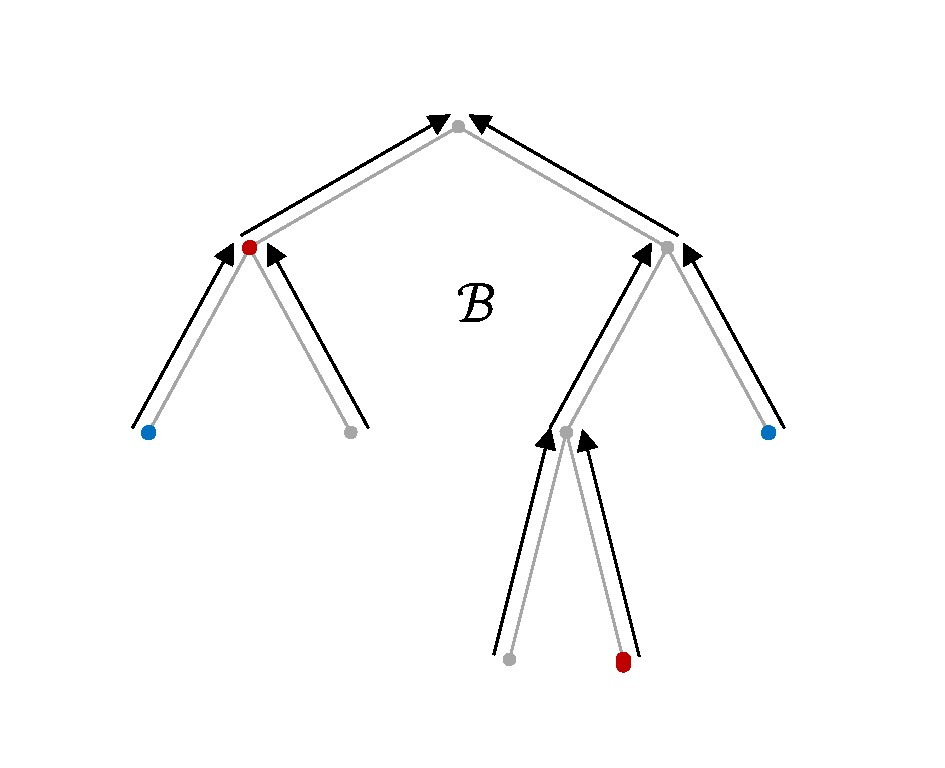
\includegraphics[trim={1.8cm 1.4cm 1.9cm 1.9cm}, clip,width=0.42\linewidth]{img/tree_2}
	\hfill
	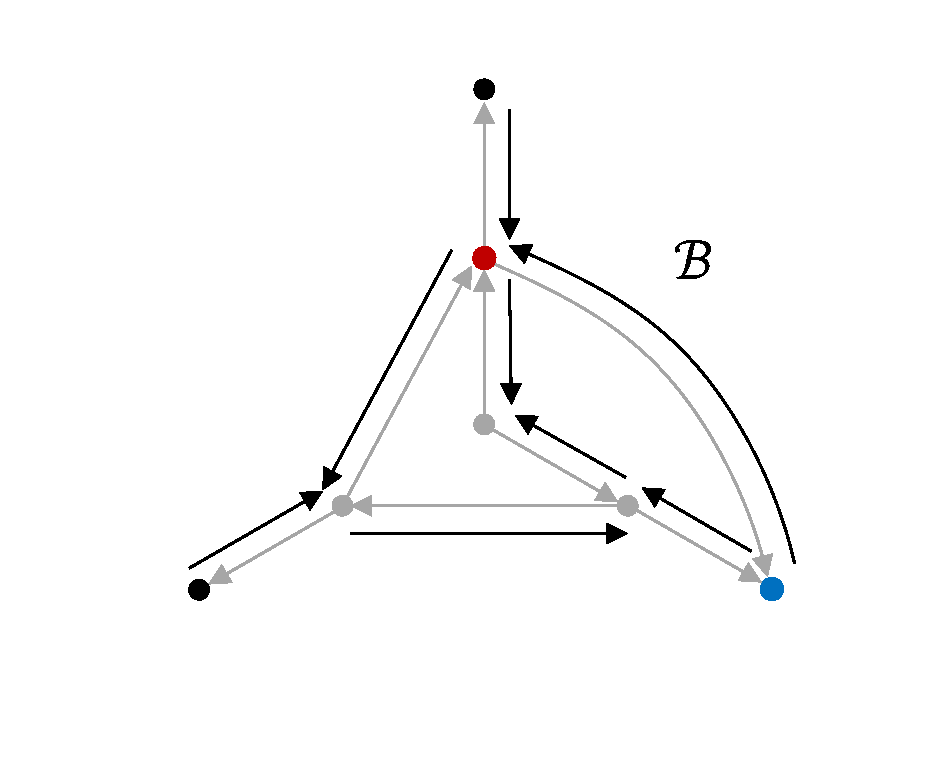
\includegraphics[trim={1.8cm 1.4cm 1.9cm 1.9cm}, clip,width=0.46\linewidth]{img/graph_2}
	\caption{Depiction of the Bellman backup operators $B$ and $\cB$.}
\end{figure}

This Bellman Operator $\cB$ was already used in the \texttt{OPD} algorithm \citet{hren2008optimistic}
Define $L_n, U_n$.\todo{Etoffer}

\begin{algorithm}
	\caption{The \emph{Optimistic Planning for Deterministic Systems} (\OPD) algorithm from \citep{hren2008optimistic}.}
	\label{alg:opd}
	\DontPrintSemicolon
	\For{each iteration $n$}{
		Compute the bounds $L_n = B_n^\infty(0)$ and $U_n = B_n^\infty(V_{\max})$.\; 
		
		$\hat{a}_n$ = $\emptyset$\;
		\While{$\hat{a}_n\in\mathring{\Tau}_n$}{
			$\hat{a}_n\gets \displaystyle\argmax_{a'\in \hat{a}_n A} r(a') + \gamma U(a')$ \Comment*[r]{Optimistic sampling rule}
		}
		\For(\Comment*[f]{Node expansion}){action $a\in A$}{
			Simulate $r, s' \sim \probability{r, s' \condbar s(\hat{a}_n), a}$.\;
			Add a new leaf $\hat{a}_n a$ to $\Tau_{n+1}$, with associated reward $r$.
		}
	}
	\Return $\displaystyle\argmax_{a\in A} r(s, a) + \gamma L(a)$. \Comment*[r]{Conservative recommendation rule}\;
\end{algorithm}

Note that $B^\infty$ actually converges in a finite time $d_n$, where $d_n$ is the depth of $\Tau_n$. Indeed, since the updates only travel the tree upward, once the information from the deepest leaf has been propagated up to the root, the obtained bound is invariant by $B$.

Likewise, we propose \autoref{alg:gbop} which follows the same approach, but on a graph structure.

\begin{algorithm}
	\caption{Our proposed \emph{Graph-Based Optimistic Planning} algorithm.}
	\label{alg:gbop}
	\DontPrintSemicolon
	\For{each iteration $n$}{
		Compute the bounds $\cL_n = \cB_n^\infty(0)$ and $\cU_n = \cB_n^\infty(V_{\max})$.\; 
		
		$\hat{s}_n$ = $s_0$\;
		\While{$\hat{s}_n\in\mathring{\cG}_n$}{
			$\hat{s}_n\gets \displaystyle\argmax_{s'} r(s, a) + \gamma \cU(s')$ \Comment*[r]{Optimistic sampling rule}
		}
		\For(\Comment*[f]{Node expansion}){action $a\in A$}{
			Simulate $r, s' \sim \probability{r, s' \condbar s, a}$.\;
			Get or create a node $s'$ in $\cG_{n+1}$, and add the transition $(s,a) \rightarrow s', r$.
		}
	}
	\Return $\displaystyle\argmax_{a\in A} r(s,a) + \gamma \cL(s(a))$. \Comment*[r]{Conservative recommendation rule}
\end{algorithm}

Though Algorithms \ref{alg:opd} and \ref{alg:gbop} look very similar, we claim that...

\section{Analysis} 

Comparing Algorithms \ref{alg:opd} and \ref{alg:gbop} directly is difficult since the two algorithms do not involve the same structures, which entails implicit differences in their behaviours. In order to leverage the previous analyses of regret bounds, we need to frame our \autoref{alg:gbop} as a tree-based planning algorithm and make these differences explicit. To account for the difference between the Bellman operators $B$ and $\cB$, we represent $\cB$ as tree backup $B$ augmented with \emph{merge} operator $M$, which enforces every node in the tree with similar states to share the same value.

First, we recall the analysis of \OPD.

\subsection{Background on the sample complexity of \OPD}

\begin{definition}[Sequence values]

%
%The value of a \textbf{state} $s\in S$ is
%\begin{equation}
%    V(s) = \max_{a\in A^\infty} R(s, a)
%\end{equation}

The value of a finite \textbf{sequence} of actions $a\in A^h$ is:
\begin{equation}
\label{eq:state_value}
    V(a) = R(s_0,a) + \gamma^{h} V(s(a)),
\end{equation}
where $R(s, a) = \sum_{t=0}^{h-1} \gamma^t r(a_{1:t})$ is the return of the sequence $a$ starting from the state $s$.
\end{definition}

The state-value bounds $L,U$ induces bounds $L^a, U^a$ for values of sequences of actions $a\in A^h$ defined as:
\begin{equation}
\label{eq:sequence_value}
\underbrace{R(a) + \gamma^{h} L(a)}_{L^a(a)} \leq V(a) \leq \underbrace{R(a) + \gamma^{h} U(a)}_{U^a(a)}
\end{equation}
%\end{definition}


Optimistic planning algorithms leverage bounds $L_n, U_n$ available at iteration $n$ to  \todo{where ?}
\begin{equation}
\label{eq:sampling_rule}
\hat{a}_n \in \argmax_{a\in\cL_n} U_n^a(a),
\end{equation}
and a conservative recommendation rule:
\begin{equation}
\label{eq:recommendation_rule}
a_n \in \argmax_{a\in\cL_n} L^a_n(a)
\end{equation}


\begin{definition}[Difficulty measure]
We define the problem-dependent measure $\hlrb{\kappa}$ as$$\hlrb{\kappa} = \limsup_{h\rightarrow\infty} |\hlrb{\Tau_h^\infty}|^{1/h}$$ 
% the smallest quantity such that $|\Tau_h^\infty| = \hlrb{\cO(\kappa^h)}$, 

%\oam{Notation $\cO()$ is slightly ambiguous here. Mention this is with respect to $h\to\infty$?}
%\el{OK. In OLOP they define it differently: $\kappa = \limsup_{h\rightarrow\infty} |\Tau_h^\infty|^{1/h}$, which is more explicit. But then you can only conclude that $\forall \kappa'>\kappa$, the regret bound holds with $\kappa'$, which feels a little more complicated to read. But it is actually closer to our Theorem 3 so it might be better?}
%\oam{Ok. The more precise the better.}

where $\hlrb{\Tau^\infty}$ is the subtree of near-optimal nodes $$\hlrb{\Tau_h^\infty} = \left\{a\in A^h: V^*-V(a) \leq \frac{\gamma^h}{1-\gamma}\right\}.$$
\end{definition}
\noindent\fbox{%
	\parbox{\textwidth}{%
\begin{theorem}[Regret bound of \texttt{OPD}]
\label{thm:regret-opd}The action $a_n$ recommended by \texttt{OPD} has a simple regret bounded by:
\begin{align*}
r_n = \cO\left( n^{-\log \frac{1}{\gamma}/\hlrb{\log\kappa}}\right).
\end{align*}
\end{theorem}
}}

\oam{Add intuition about $\kappa$ ? When is it typically big, small ?
Recall some examples from literature.}
\oam{Add discussion regarding literature scarcity on the topic}
\el{OK.}

\subsection{Motivation for an improved regret bound}

The trivial bound used in \texttt{OPD} does not make use of all the available information in $\Tau_n$. Assume that we had access to some tighter bounds $L,\,U$ provided by an oracle: $$0\leq L\leq V\leq U\leq V_{\max}.$$

\begin{definition}[A finer difficulty measure]
We define the near-optimal branching factor \emph{according to the bounds $L,\,U$} as $$\hlbb{\kappa(L,U) \eqdef \limsup_{h\rightarrow\infty} \left|\Tau_h^\infty(L,U)\right|^{1/h}}\in(1, K],$$ where
\begin{equation}
     \hlbb{\Tau_h^\infty(L,U)}=\left\{a\in A^h: V^* - V(a)\leq \gamma^{h}(U(a)-L(a))\right\}.
\end{equation}

\end{definition}

\begin{lemma}This branching factor shrinks as the bounds $L,\,U$ get tighter:
\[L_2\leq L_1\leq V\leq U_1\leq U_2\implies \kappa(L_1,U_1) \leq \kappa(L_2,U_2).\]
In particular, $\hlbb{\kappa(L,U)} \leq \hlrb{\kappa}$.
\end{lemma}


\noindent\fbox{%
	\parbox{\textwidth}{%
\begin{theorem}
\label{thm:regret-bound-U}
Let $L \leq V\leq U$ consistent bounds, then planning with $L^a,\,U^a$ yields the following simple regret bound: %$\forall \kappa>\kappa(U)$,
\begin{equation*}
r_n = \cO\left(n^{-\log \frac{1}{\gamma}/\hlbb{\log \kappa(L,U)}}\right).
\end{equation*}
\end{theorem}
}}

\el{Ici: expliquer que le thm 2 nous dit qu'on peut potentiellement avoir une amélioration mais qu'il ne dit pas comment obtenir des bornes U, L. Pour cela la section 3, on détaille une méthode pour construire une séquence de bornes de plus en plus fines. Ajouter un renvoi au résultat final Thm3}


\subsection{Merging the states}

\begin{definition}
	We say that a lower-bound $L$ and an upper bound $U$ are \emph{consistent} if they are respectively non-decreasing and non-increasing along sequences of actions:
	\begin{align*}
	\forall a\in\Tau_n\setminus\cL_n, \quad &L(a) \leq \max_{b\in A} r(ab) + \gamma L(ab)\\
	&U(a) \geq \max_{b\in A} r(ab) + \gamma U(ab)
	\end{align*}
\end{definition}

\begin{lemma}
	$B$ verifies $B^{\infty}=B^{d_n}$, $B$ preserves consistency, and $B$ tightens consistent bounds $L,U$:
	\begin{equation*}
	L\leq V \leq U \implies L \leq B(L) \leq V \leq B(U) \leq U
	\end{equation*}
\end{lemma}

As shown in \ref{fig:bellman}, in a tree the Bellman operator $B$ only propagates the information upward, and the leaves cannot be updated.

Applying $B$ is \emph{not valuable} on its own for planning with \eqref{eq:sampling_rule}, since  $B(V_{\max})$ and $V_{\max}$ coincide on $\cL_n$.

\begin{definition}[Merge operator]
If several sequences $a'\in\Tau_n$ all lead to the same state $s$, their respective bounds must hold simultaneously. This suggests a merge operator $M$ as:
    \begin{align}
    \label{eq:aggregation}
        \forall a\in\mathcal{T}_n, \qquad &M_n^-(L)(a) = \max_{a'\in \cN_n(a)} L(a'),\qquad M_n^+(U)(a) = \min_{a'\in \cN_n(a)} U(a').                                   
    \end{align}
\end{definition}

\oam{This is ambiguous $M(f)$ is either LHS or RHS of \eqref{eq:aggregation}. How do you decide which one? Don't you need some $M_{+}$and $M_{-}$?
}
\el{Right, I can't find a notation that is both rigorous and simple. Introducing A+ and A- is pretty good but we need to keep this distinction everywhere, which is a bit tedious. Maybe A could operate on pairs (L,U) of bounds instead? Not great either...}

\begin{figure}[H]
	\centering
	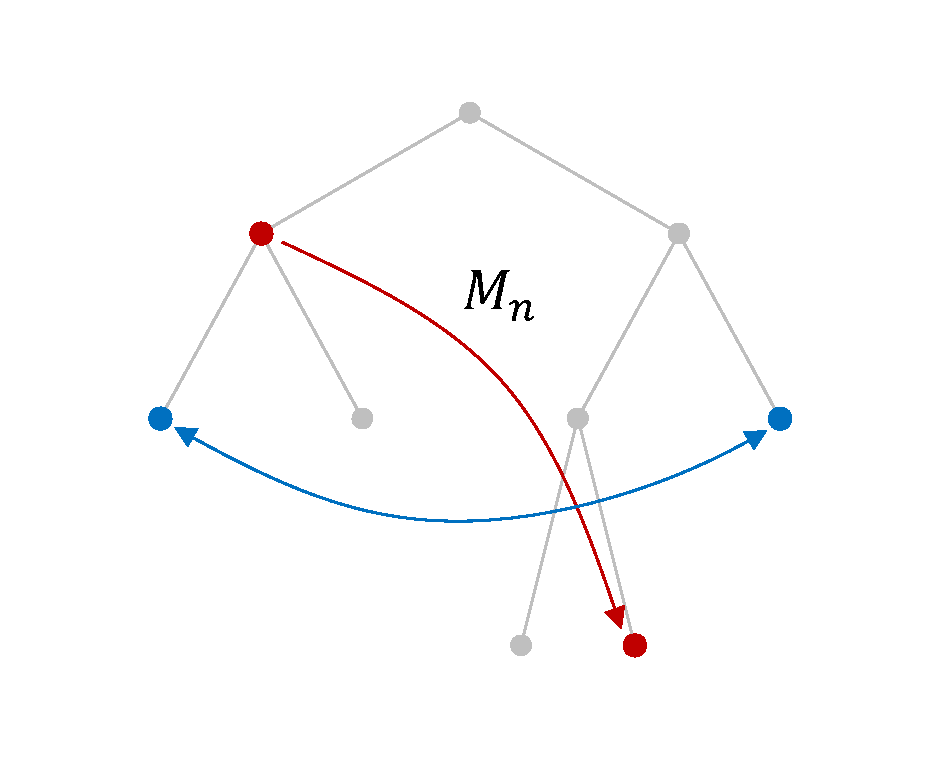
\includegraphics[trim={1.8cm 1.8cm 1.9cm 1.8cm}, clip,width=0.4\linewidth]{img/tree_3}
	\caption{Depiction of the aggregation operator $M$. Nodes can be updated anywhere in the tree $\Tau_n$, and in particular its leaves $\cL_n$.}
\end{figure}

\begin{lemma}
We have $M^2=M$, $M$ preserves consistency, and tightens bounds:
\begin{equation*}
    L\leq V \leq U \implies L\leq M^-(L) \leq V \leq M^+(U) \leq U
\end{equation*}
\end{lemma}

At this stage, we have defined two operators $M$ and $B$ that operate on bounds $f$ and can only tighten them.


\begin{remark}[Interplay of backups and aggregations]
As observed earlier, the sampling rule \eqref{eq:sampling_rule} only depends on the value of $U$ at the leaves $\cL_n$, which makes applying $B$ alone useless since information only travels upwards in the tree $\Tau_n$. Conversely, applying $M$ can update the value of any node in the tree $\Tau_n$, including the leaves $\cL_n$. These tightened bounds at the leaves can then be propagated upward with Bellman backups $B$ to update inner nodes, which can in turn be aggregated with other leaf nodes, and so forth.
\end{remark}

This suggests an alternating procedure of aggregations $M$ and backups $B$, whose convergence must be studied.

\begin{proposition}[Contractivity of $MB$]
\label{prop:contractivity}
$M B$ a $\gamma$-contraction.
\end{proposition}

We can perform a fixed-point iteration of alternating backups and aggregations starting from the trivial bounds $L_0=0$, $U_0 = V_{\max}$.

\begin{equation}
    \label{eq:recursion}
    L^k = (M B)^k(0), \qquad
    U^k = (M B)^k(V_{\max})
\end{equation}
$(U^k)$ (resp. $(L^k)$) is non-increasing (resp. non-decreasing) and converges at a rate $\gamma^k$, but can converge in infinite time whenever there is a loop, as shown in \autoref{sec:convergence}. We can decide to stop whenever a desired accuracy is reached: 

\begin{proposition}[Early stopping]
\label{prop:early-stopping}
Provided that
\[\forall a\in\Tau_n,\; |U^{k+1}(a) - U^k(a)| \leq \epsilon (1-\gamma)\gamma^{-h(a)-1},\]
then the sequence upper-bound $U^{a,\infty}$ is approximated by $U^{a,k+1}$ with an accuracy of $\epsilon$.
\end{proposition}

\paragraph{Pruning of leaves}

Another observation can be made in the case where two nodes $a_1,a_2\in\Tau_n$ lead to the same state $s$:
\begin{proposition}[Pruning rule]
\label{prop:pruning}
Let $a_1,a_2\in\Tau_n$ such that state $s(a_1) = s(a_2) = s$ and $U = M(U) \geq V$ an aggregated upper-bound. 
\begin{equation}
\label{eq:pruning}
    \text{If } h(a_2) \geq h(a_1) \text{ and } U^a(a_2) \geq U^a(a_1)
    \text{, then }V(a_2) \geq V(a_1)
\end{equation}

In particular, there is no need to ever expand the node $a_1$.
\end{proposition}

We propose that at each step, we detect such pairs $a_1, a_2$. Whenever $a_1$ is a leaf, we can remove it from the set $\cL_n^-\subset \cL_n $ of candidates for expansion.

\begin{figure}[H]
	\centering
	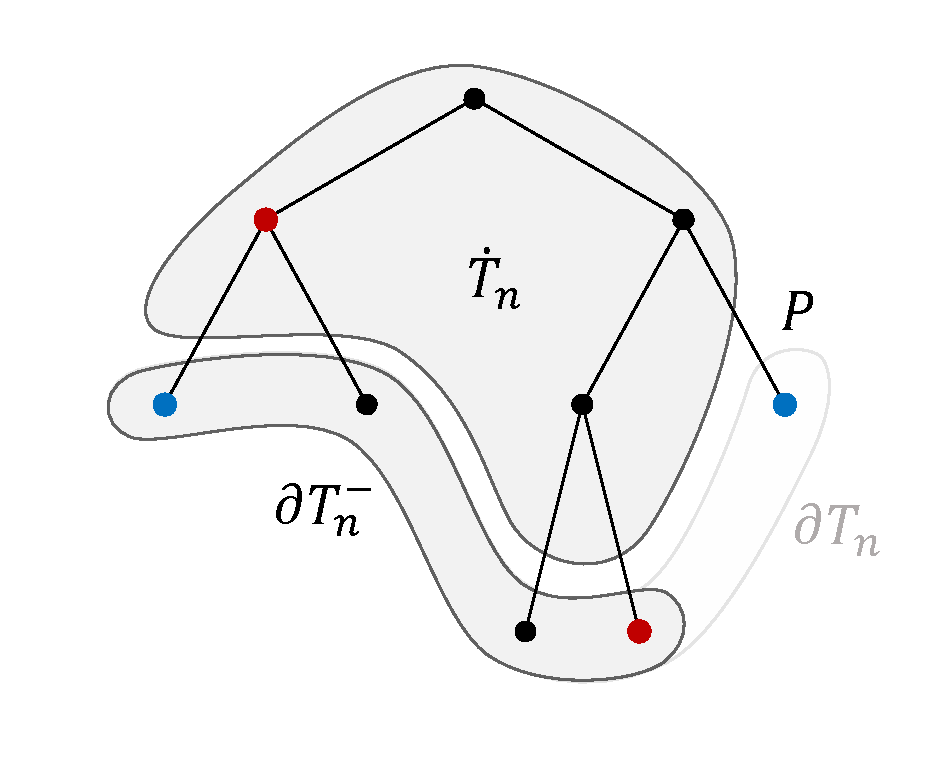
\includegraphics[trim={1.8cm 1.4cm 1.9cm 1.1cm}, clip, width=0.4\linewidth]{img/tree_4}
	\caption{Depiction of the leaves pruning operator $\cP$. A leaf verifying the criterion of \autoref{prop:pruning} is removed from the set of leaves candidate to expansion.}
\end{figure}

The full algorithm is described in \autoref{alg:state-aware}.\\
\begin{algorithm}[H]
	\caption{State-aware planning}
	\label{alg:state-aware}
	\SetAlgoLined\DontPrintSemicolon
	\For{iteration $n$}{
		\nl Given $\Tau_n$, compute $L_n = (M_n^-B_n)^\infty(0)$ and $U_n = (M_n^+B_n)^\infty(V_{\max})$ with \eqref{eq:aggregation} and \eqref{eq:bellman}.\;
		\nl Select the optimistic sequence of actions $\hat{a}_{n}$ from \eqref{eq:sampling_rule}.\;
		\For(\tcp*[h]{Expand the corresponding leaf node}){action $a\in A$}{
			Add the child $\hat{a}_{n}a$ to the tree $\Gamma_{n+1}$ and observe its reward.
		}
		\nl Prune the tree: $\cL_{n+1}^- = \cP(\cL_{n+1})$.\;
	}
	\Return the recommendation $a_{n+1}$ from \eqref{eq:recommendation_rule}.\;
\end{algorithm}

\subsection{Main result}

In \autoref{thm:regret-bound-U}, we assumed that some bounds $L,\,U$ were revealed by and oracle and available from the onset for planning. In \autoref{alg:state-aware}, we instead built a non-increasing (in the sense of inclusion) \emph{sequence} of bounds $(L_n,U_n)_{n\geq 0}$, i.e. that verify $0\leq \dots\leq L_{n-1}\leq L_n\leq V\leq U_n\leq U_{n-1}\leq \dots\leq V_{\max}$.

We can consider the sequence $\kappa_n = \kappa(L_n, U_n)$. It is non-increasing and lower-bounded by $1$, thus converges. Let $\hlgb{\kappa_\infty = \lim_{n\rightarrow\infty} \kappa(L_n, U_n)} \in[1,K]$.

\begin{proposition}
	\el{We need to convey the intuition that $\kappa_\infty$ will be much lower than $\kappa$ in problems where trajectories overlap a lot, for instance problems where two actions cancel-each other out (e.g. moving left or right), or when the outcome of several actions does not depend on the order (e.g. placing pawns on a board game). But this property concerns $\kappa_\infty$ thanks to the aggregation operator providing the bounds $L_n, U_n$, I do not think we can provide more intuition with arbitrary bounds $L,U$.}
\end{proposition}

\begin{theorem}
\label{thm:regret-state-aware}
The \autoref{alg:state-aware} enjoys the following regret bound: 
\begin{align*}
\forall \hlgb{\kappa' > \kappa_\infty}, \quad r_n = \cO\left(n^{-\log \frac{1}{\gamma}/\hlgb{\log \kappa'}}\right)
\end{align*}
\end{theorem}

\oam{What is a bit odd is that
nowhere in the document you seem to define precisely the $L$ and $U$ bounds. I think you should discuss a full example, with precise values for each quantity.
Perhaps also provide a complete pseudo-code of the whole procedure (at least in appendix).
}
\el{The pseudocode is provided in Algorithm 1, where the bounds $L_n, U_n$ used are written line 1. But it could be made clearer after Proposition 1.}
\oam{Indeed, it is a bit unclear. Especially, I see the definition of $M$ and $\cB$, but not of $M_n$ and $\cB_n$. Also the precise meaning of $M\cB$ is slightly ambiguous due to the ambiguous definition of $M$. Perhaps you can refer to the equation numbers/defs where each term is defined.
}
\el{The $n$ comes from the fact that A and B actually depend on $\Tau_n$, but I omitted it everywhere for simplicity. I will add a remark on that when I introduce the operators. I will add more references.}


\subsection{Illustrative example}
\label{sec:illustrative-example}
We consider a toy MDP $\cM$ shown in \autoref{fig:mdp}. The transitions are described visually while the rewards are defined as follows: let $0\leq r^*\leq \gamma$, and $ r^- = r^* - \frac{\gamma}{1-\gamma} S$, $r^+ = r^* + S$ with $S = r^*\left(\frac{1}{\gamma} - 1\right).$ Note that the choice ensures that $r^*, r^-, r^+$ and $S$ are all in $[0, 1]$.

\begin{figure}[htp]
    \centering
    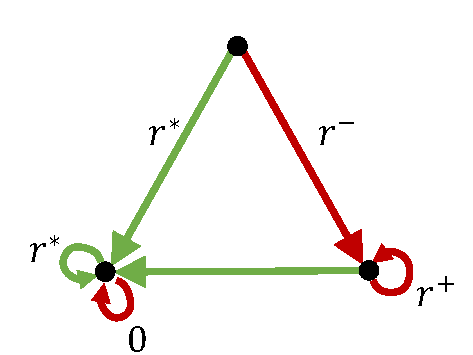
\includegraphics[width=0.5\textwidth]{img/mdp.pdf}
    \caption{A toy MDP with three states and $K \geq 2$ actions. We start in the top state. The first action $a_1$ is represented by \textcolor{OliveGreen}{green} arrows, and all other actions $a_2, \dots, a_K$ are represented by \textcolor{red}{red} arrows. The rewards are shown next to the transitions.}
    \label{fig:mdp}
\end{figure}

\begin{proposition}[Comparison of branching factors]
\label{prop:illustrative-example}
The MDP $\cM$ verifies:
\begin{enumerate}
    \item $\hlrb{\kappa = K-1}$;
    \item $\hlgb{\kappa_\infty = 1}$.
\end{enumerate}
In particular, if $K\geq 3$ then $\hlgb{\kappa_\infty} < \hlrb{\kappa}$.
\end{proposition}

\oam{Explain what is natural/expected in this result.  What is perhaps surprising/novel/non-trivial? What impact on practitioners? }
\oam{Explain here what you used precisely for bounds $U,L$ in these implementations}

\section{Extension to stochastic systems}

Whenever a planning algorithm is based on bounds over the values, our approach can be applied to tighten these bounds while preserving their validity. In particular, when the rewards and/or transitions are stochastic, many algorithms rely on confidence intervals to build statistical bounds on the values that hold with high probability.

By tightening the bounds, we preserve the guarantees that rely on their validity and rate of convergence. 

\subsection{Stochastic rewards}

KL-OLOP

\subsection{Stochastic dynamics}

MDP-GapE ?

Other closed loop algorithms are not runnable, except BRUE which is not optimistic and does not involve bounds.

\section{Numerical Experiments}

\oam{Better explain the figures shown in this section}

\oam{On top of the illustrative pictures, would it be possible to compute some simple score, say 
for each $k\in\mathbb{N}$,  count the number $o_k$ of occupancies at distance $k$ from the goal, then look at a weighted sum, $\sum_{k} w_k o_k$,
where $w_k$ is decreasing ($1/k$, or $\alpha^k$, etc.) ?
}
\el{Alright. Why do you want the weights to decrease with distance?}

\el{Do we need an example (e.g. 1 state 2 actions) to show that even in the cases where $\kappa=\kappa_\infty$ asymptotically, the non-asymptotic behaviour of state-aware planning can be much better?}
% \paragraph{Illustrative example}
% We consider the example problem of \autoref{sec:illustrative-example} with $r_1=0$ and $r_2 = 0.7$. As expected from \autoref{prop:illustrative-example}, the tree expanded by \texttt{OPD} is quite balanced, even with such a dense reward and important gap. In contrast, The state-aware planner never expands a suboptimal node.
% \begin{figure}[H]
%     \centering
%     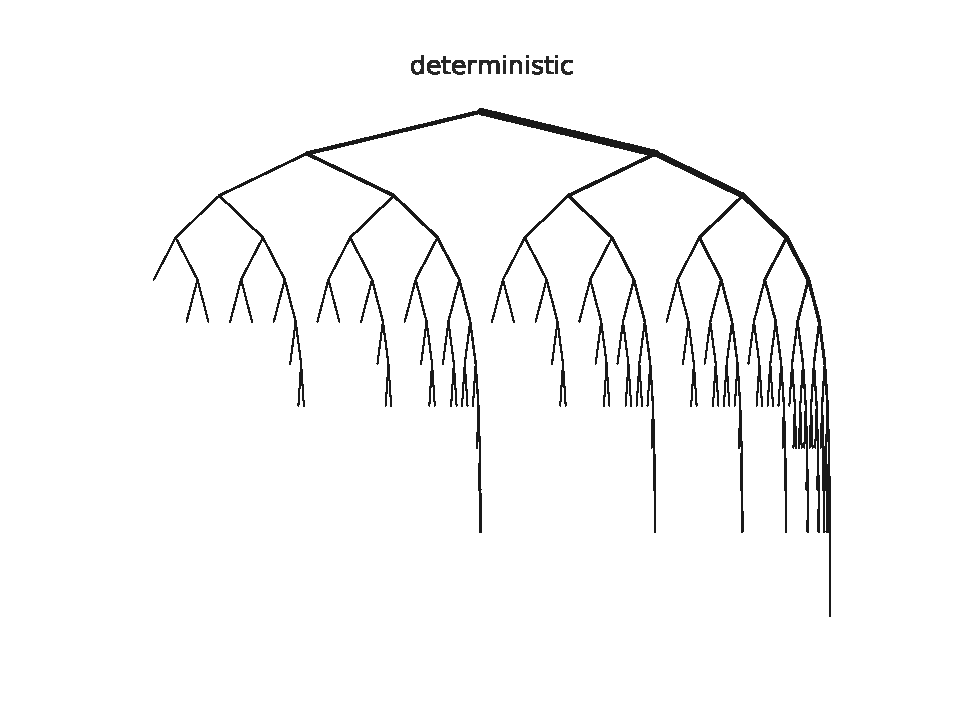
\includegraphics[width=0.49\textwidth]{img/bandit_deterministic.pdf}
%     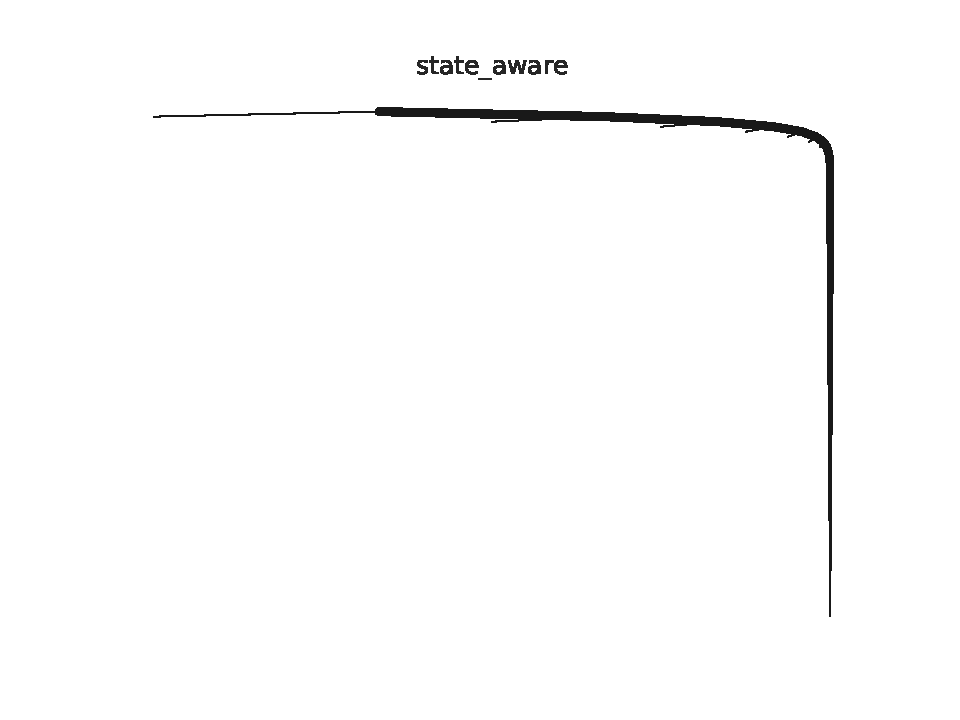
\includegraphics[width=0.49\textwidth]{img/bandit_state_aware.pdf}
%     \caption{Trees expanded for $n = 200$, $\gamma=0.99$}
%     \label{fig:bandit_trees}
% \end{figure}

\paragraph{Gridworld}

The reward is a paraboloid centred at $(10, 10)$ with length-scale of 5:  $r(x, y) = 1 - \frac{1}{5^2}((x-10)^2 + (y-10)^2)$ clipped to [0, 1].

\begin{figure}[H]
    \centering
    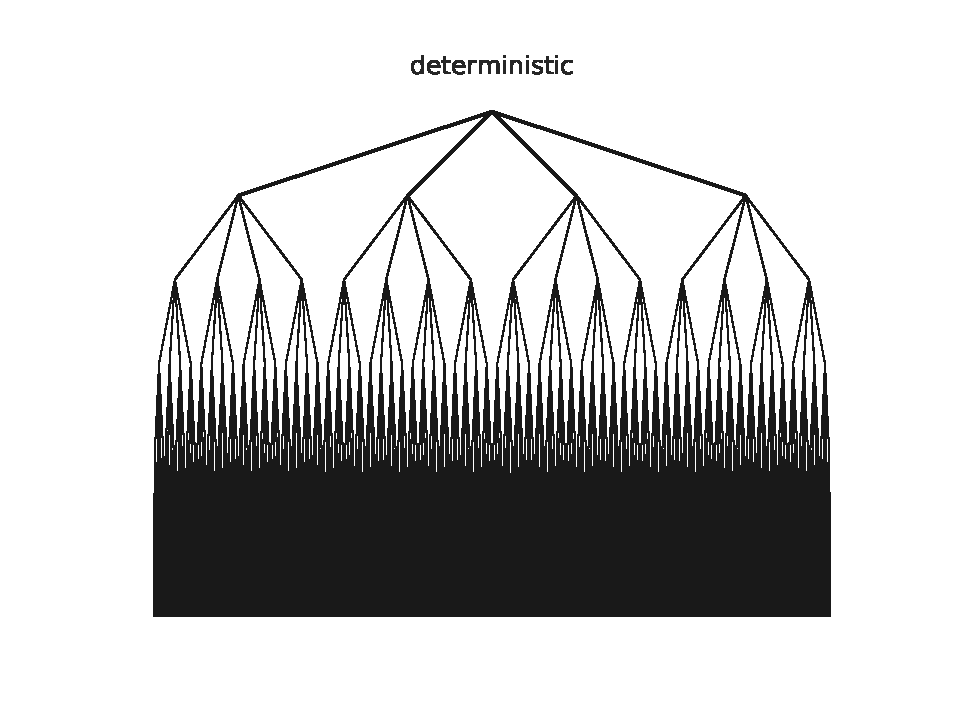
\includegraphics[width=0.32\textwidth]{img/4_deterministic.pdf}
    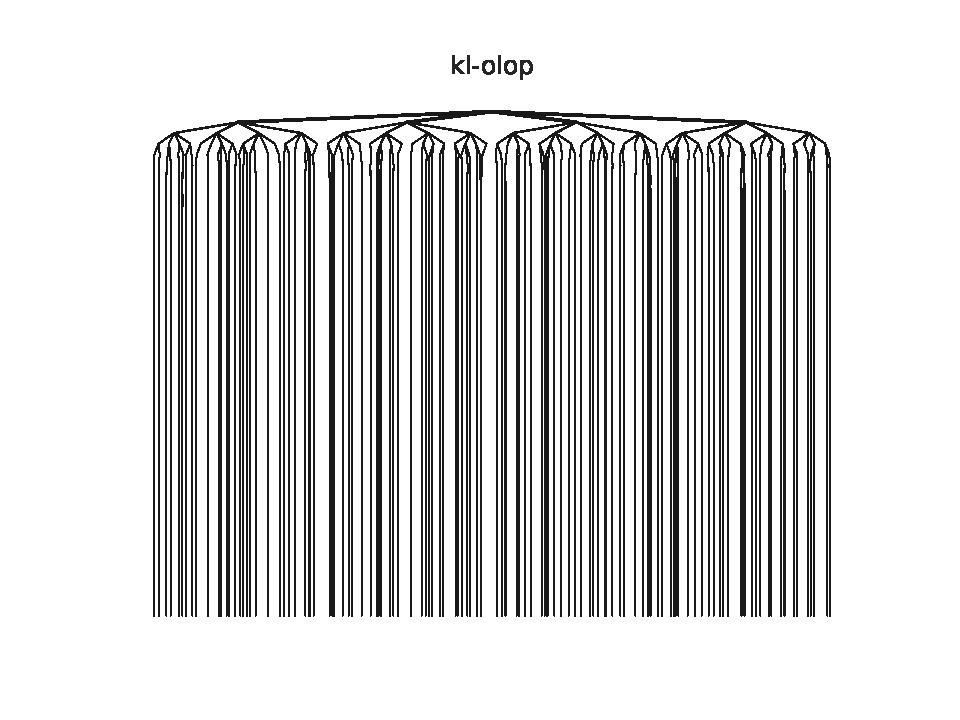
\includegraphics[width=0.32\textwidth]{img/4_kl-olop.pdf}
    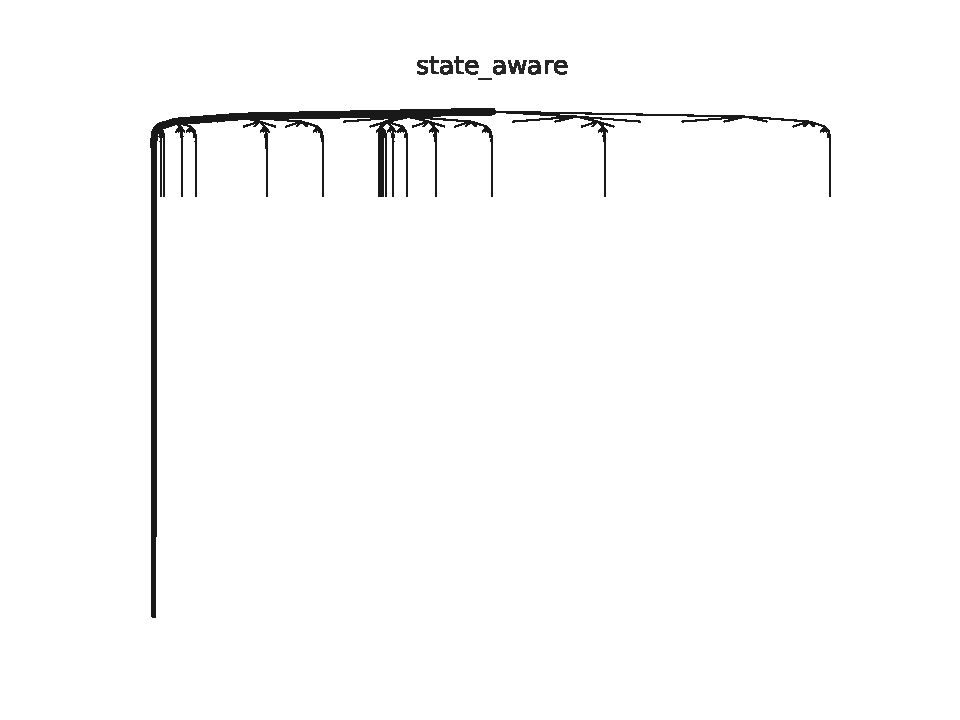
\includegraphics[width=0.32\textwidth]{img/4_state_aware.pdf}
    \caption{Trees expanded for $n = 5460$, $\gamma=0.95$}
    \label{fig:gw4_trees}
\end{figure}
\begin{figure}[H]
    \centering
    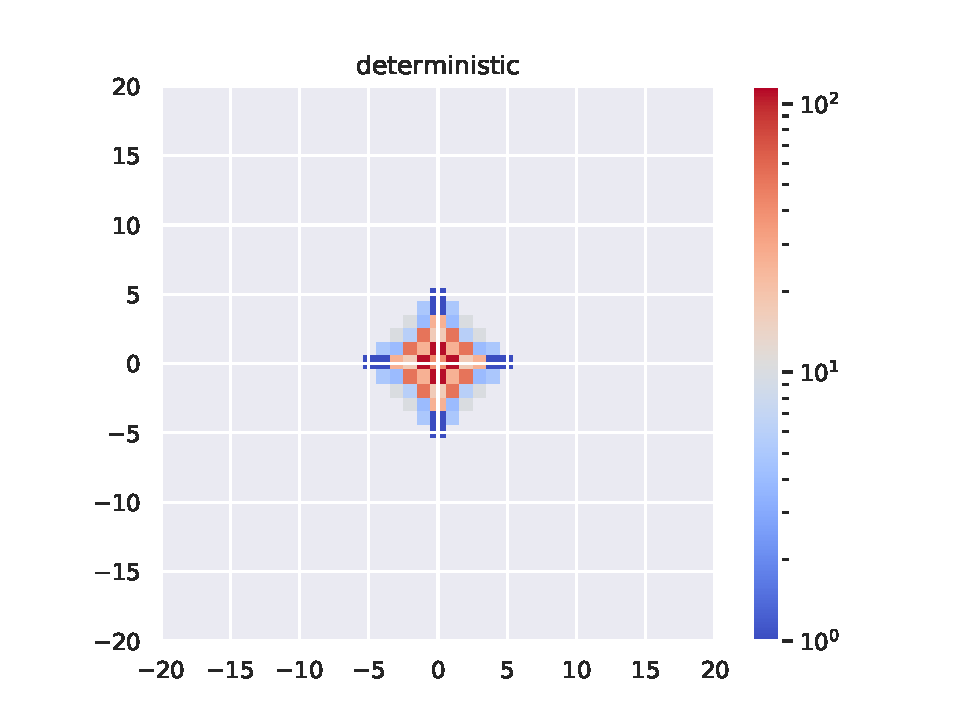
\includegraphics[width=0.32\textwidth]{img/4_occupations_deterministic.pdf}
    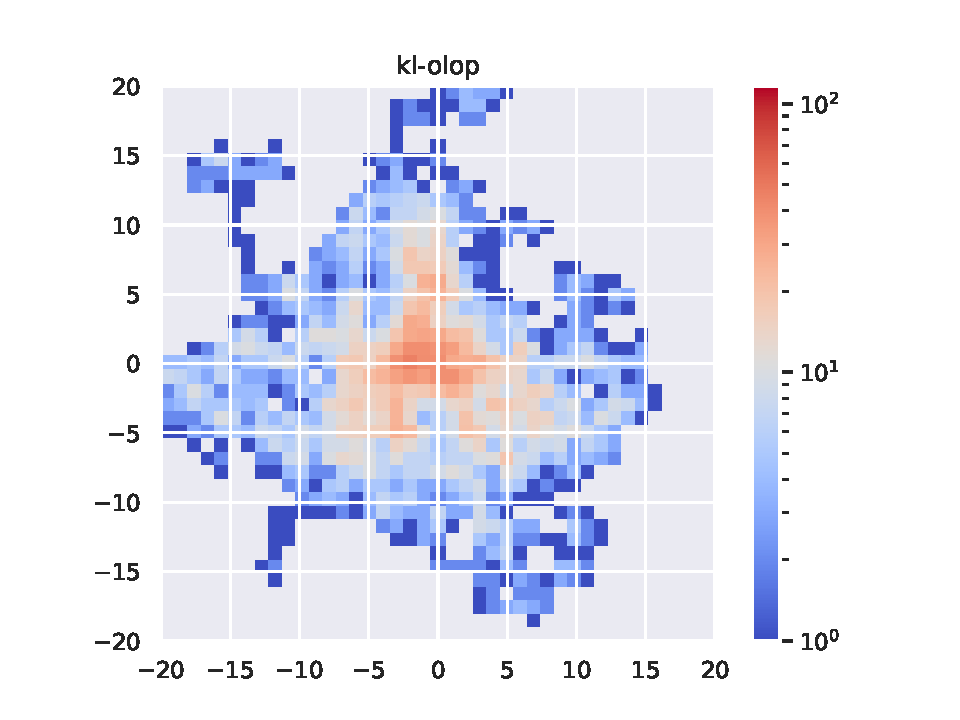
\includegraphics[width=0.32\textwidth]{img/4_occupations_kl-olop.pdf}
    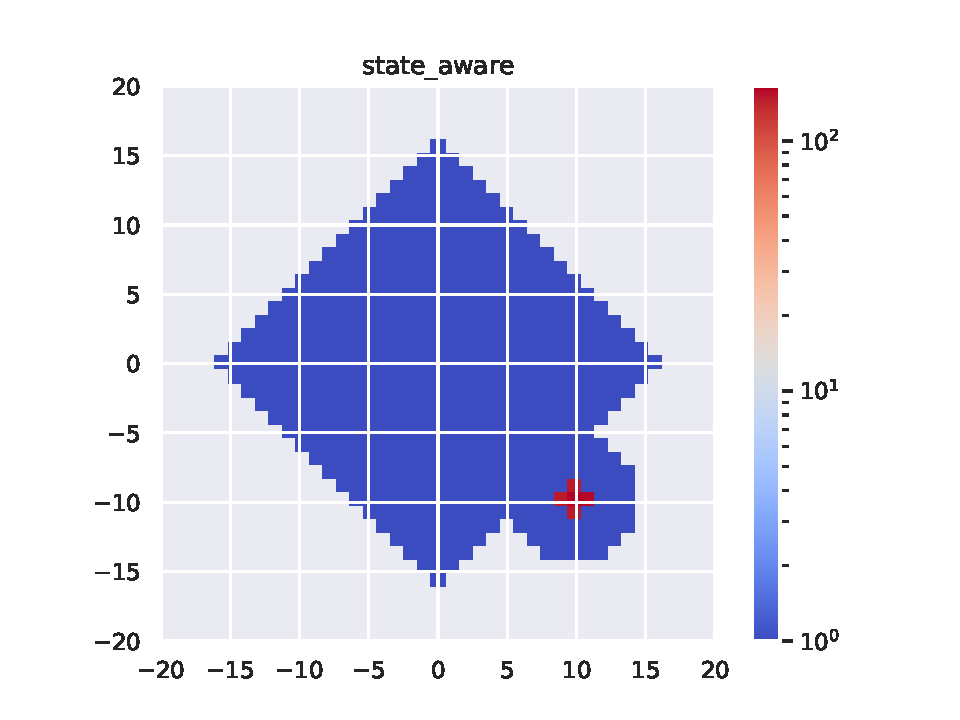
\includegraphics[width=0.32\textwidth]{img/4_occupations_state_aware.pdf}
    \caption{Number of visits for $n = 5460$, $\gamma=0.95$}
    \label{fig:gw4_visits}
\end{figure}
\begin{figure}[H]
    \centering
    % \includegraphics[width=0.49\textwidth]{img/4_updates_deterministic.pdf}
    % \includegraphics[width=0.49\textwidth]{img/4_updates_kl-olop.pdf}
    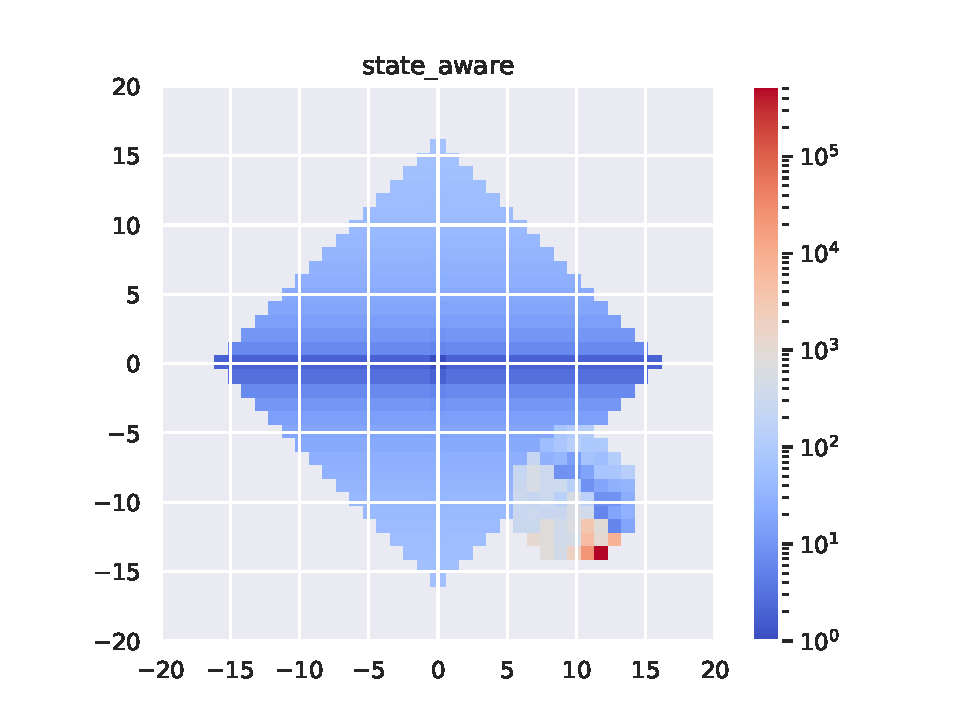
\includegraphics[width=0.7\textwidth]{img/4_updates_state_aware.pdf}
    \caption{Number of updates in the leaf expansion for $n = 5460$, $\gamma=0.95$}
    \label{fig:gw4_updates}
\end{figure}

\paragraph{Sailing}

\section*{Conclusion}


\bibliography{references}


\clearpage
\appendix

\section{Proofs}
\subsection{Proof of \autoref{thm:regret-opd}}
Sketch of proof.\\
\noindent\fbox{%
	\parbox{\textwidth}{%
		\begin{enumerate}
			\item The recommendation $a_n$ has a maximal depth $d_n$ in the tree, and its gap $r_n = V^* - V({a_n}_{1})$ is bounded by $r_n \leq \frac{\gamma^{d_n}}{1-\gamma}$. We need to relate $d_n$ to $n$.
			
			\item Each expanded node belongs to $\Tau^\infty = \bigcup_{h\geq 0} \Tau_h^\infty$, where $$\Tau_h^\infty = \left\{a\in A^h: V^*-V(a) \leq \frac{\gamma^h}{1-\gamma}\right\}.$$ Introduce the difficulty measure $\kappa$ such that $|\Tau_h^\infty| = \cO(\kappa^h)$ (the smallest).
			
			\item In the worst case, expanded nodes fully fill the depths of $\Tau^\infty$ up to $d_n$: $n = \sum_{d=1}^{d_n} n_d \leq  C\sum_{d=1}^{d_n} \kappa^d = \begin{cases}
			\cO(d_n) &\text{if $\kappa=1$}\\
			\cO(\kappa^{d_n}) &\text{else.}
			\end{cases}$\\
			Hence $r_n = \begin{cases}
			\cO(\gamma^n) &\text{if $\kappa=1$}\\
			\cO(\gamma^{\frac{\log n}{\log \kappa}}) = \cO(n^{-\frac{\log 1/\gamma}{\log \kappa}}) &\text{else.}
			\end{cases}$
		\end{enumerate}
	}%
}

\subsection{Proof of \autoref{thm:regret-bound-U}}
In this proof, we temporarily assume that $U=B(U)$ and $L=B(L)$. We follow the same steps as in the proof of the regret of \texttt{OPD}.

\begin{remark}
It does not hold anymore that $a_n$ must be of maximal depth $d_n$.  This is due to the fact the exploration bonus $\gamma^h U(a)$ is not depth-wise constant: consider two nodes $a,b$ at the same depth with $R(a) > R(b)$. In \texttt{OPD}, both get the same bonus $\gamma^h/(1-\gamma)$, and the node $a$ is expanded first. But with the local bonus, $b$ could be expanded in priority rather than $a$, if its own bonus is sufficiently higher than that of $a$, precisely if $R(a)+\gamma^h U(a) < R(b)+\gamma^h U(b)$. For instance, $U(a)=0$ when $a$ is known to be a terminal state while $b$ can lead to future rewards. If after expanding and exploring the subtree of $b$ we find out that $V(b) = 0$, we still return the recommendation $a$, which is of non-maximal depth.
\end{remark}

The regret bound still holds, however. First, notice that:
\begin{lemma}
\label{lemma:expansion-bound}
Whenever a node $a$ of depth $h$ is expanded by the optimistic algorithm, its first action $a_1$ enjoys a simple regret $V(a^*)-V(a_1) \leq \gamma^h(U(a)-L(a))$. 
\end{lemma}
\begin{proof}
Let $t$ be the time of expansion of $a$, it holds that $U^a_t(b) \leq U^a_t(a)$ for all $b\in \cL_t$, in particular those in a branch starting by an optimal action $a^*$. Since $U=B(U)$ and $L=B(L)$, we also have $U^a_t(a^*) = \max_{b\in a^*A^*} U^a_t(b) \leq U^a_t(a)$, and $L^a_t(a_1) = \max{b\in a_1 A^*} L^a_t(b) \geq  L^a_t(a)$. Thus, $V(a^*)-V(a_1) \leq U^a_t(a^*) - L^a_t(a_1) \leq U^a_t(a) - L^a_t(a) = \gamma^h(U(a)-L(a))$.
\qed\end{proof}
 
\begin{lemma}
The recommended action $a_n$ has a simple regret $r_n \leq \frac{\gamma^{d_n}}{1-\gamma}$, where $d_n$ is the maximal depth of $\Tau_n$.
\end{lemma}
\begin{proof}
Let $i$ a node of maximal depth $d_n$, and consider the recommended node $a_n$ at time $n$, of depth $d$. In particular, $L^a_n(a_n) \geq L^a_n(i)$, and since $(L^a_t)_t$ is non-decreasing we also have $L^a_n(i) \geq L^a_t(i)$. At the time $t$ when $i$ is expanded, we have $U^a_t(a_n) \leq U^a_t(i)$, and since $(U^a_t)_t$ is non-increasing we also have $U^a_n(a_n) \leq U^a_t(a_n)$. We can conclude with \autoref{lemma:expansion-bound} applied to $a_n$: $r_n \leq \gamma^d(U(a_n)-L(a_n) = U^a_n(a_n) - L^a_n(a_n)  \leq U^a_t(a_n) - L^a_n(i) \leq U^a_t(i) - L^a_t(i) = \gamma^{d_n}(U(i) - L(i)$, which yields the claimed bound since $U(i) - L(i) \leq V_{\max}-0$.
\qed\end{proof}

\begin{lemma}
\label{lemma:expansion-tree}
Every node expanded by \eqref{eq:sampling_rule} is in $\Tau^\infty(L,U) = \bigcup_{h\geq 0} \Tau^\infty_h(L,U)$.
\end{lemma}
\begin{proof}
Let $a$ be a node of depth $h$ expanded at round $n$, then $U^a_n(a) \geq U^a_n(b)$ for all $b\in\cL_n$. Thus, since $U = B(U)$, we have $U^a(a) = B(U)^a(\emptyset) = B(U)(s_0) \geq V(s_0) = V^*$. Thus, $V^* - V(a) \leq U^a(a) - L^a(a) = \gamma^h(U(a) - L(a))$.
\qed\end{proof}

Finally, we can move on to the proof of \autoref{thm:regret-bound-U}.
Let $n_d$ be the number of expanded nodes of depth $d$, by \autoref{lemma:expansion-tree} we have $n_d \leq |\Tau^\infty_d(L,U)| \leq C\kappa(L,U)^d$. Thus, 
\[n = \sum_{d=1}^{d_n} n_d \leq C\sum_{d=0}^{d_n} \kappa(L,U)^d = C\frac{\kappa(L,U)^{d_n+1}-1}{\kappa(L,U)-1}\]
Hence, $d_n \geq C'\frac{\log n}{\log\kappa(L,U)},$ which along with \autoref{lemma:expansion-bound} gives the claimed bound.

Note that if $L,\,U$ are consistent bounds that do not verify $L = B(L)$ and $U=B(U)$, then planning with $B(L),B(U)$ instead will yield the proved bound with a branching factor $\kappa(B(L),B(U))$, and since $L\leq B(L)\leq V\leq B(U)\leq U$ we have $\kappa(B(L),B(U)) \leq \kappa(L,U)$, which still gives \begin{align*}
r_n = \cO\left(n^{-\frac{\log 1/\gamma}{\log \kappa(L,U)}}\right);
\end{align*}

\subsection{Proof of \autoref{prop:contractivity}}
\begin{proof}
Let $U_1, U_2\in \Real^\Tau_n, a\in\Tau_n$,
\begin{align*}
    (M U_1 - M U_2)(a) &= \min_{a'\in\cN_n(a)} U_1(a') - \min_{a'\in\cN_n(a)} U_2(a') \\
    &= \min_{a'\in\cN_n(a)} U_1(a') - U_2(a^-) \\
    &\leq U_1(a^-) - U_2(a^-) \\
    &\leq \|U_1 - U_2\|_\infty
\end{align*}
where $a^-\in \argmin_{a'\in\cN_n(a)} U_2(a')$. 
Hence, $\|M U_1 - M U_2\|_\infty \leq \|U_1 - U_2\|_\infty$
\qed\end{proof}

\subsection{Proof of \autoref{prop:early-stopping}}

\begin{proof}
Let $a\in A^h$. We consider the sequence $(U^a_n)_{n\in\Natural}$.
Notice that for any $U,V\in\Real^\Tau$, we have $U^a(a)-V^a(a)=\gamma^h(U(a)-V(a))$.

Hence, if the premise holds,
\begin{align*}
    |U^a_{k+1}(a) - U^a_{k}(a)| &\leq \gamma^h\epsilon (1-\gamma)\gamma^{-h-1} = \epsilon (1-\gamma)\gamma^{-1}
\end{align*}

And then,
\begin{align*}
|U^a_{k+1}(a) - U^a_\infty(a)| &= \gamma^h |U_{k+1}(a) - U_\infty(a)|\\
&\leq \gamma^{h+1}|U_{k}(a) - U_\infty(a)| \text{ since $LA$ is a $\gamma$-contraction}\\
&\leq \gamma^{h+1}|U_{k}(a) - U_{k+1}(a)| + \gamma^{h+1}|U_{k+1}(a) - U_\infty(a)|\\
&= \gamma|U^a_{k}(a) - U^a_{k+1}(a)| + \gamma |U^a_{k+1}(a) - U^a_\infty(a)|\\
&\leq \frac{\gamma}{1-\gamma} |U^a_{k}(a) - U^a_{k+1}(a)|\\
&\leq\epsilon
\end{align*}
\qed\end{proof}

\subsection{Proof of \autoref{prop:pruning}}

\begin{proof}
Assume $h(a_2) \geq h(a_1)$.
\begin{align*}
    V(a_1) - V(a_2) &= R(a_1)- R(a_2) + \underbrace{\left(\gamma^{h(a_1)} - \gamma^{h(a_2)}\right)}_{\geq 0}V(s) \\
    &\leq R(a_1)- R(a_2) + \left(\gamma^{h(a_1)} - \gamma^{h(a_2)}\right)U(s)\\
    &= U^a(a_1) - U^a(a_2)
\end{align*}
Hence, if this last term is negative, then $V(a_1) - V(a_2)$ is as well.
\qed\end{proof}

\subsection{Proof of \autoref{thm:regret-state-aware}}

\begin{proof}
Let $\kappa'>\kappa_\infty$. Since $\kappa(L_n,U_n)\rightarrow\kappa_\infty$, there exists $n_0\in\Natural$ such that for all $n\geq n_0$, $\kappa(L_n,U_n) \leq \kappa'$.
We can show that at each iteration $n$, the expanded node must belong to $\Tau^\infty(L_n,U_n)$.
Let $n\geq n_0$, and define $d_0 = \min\{d\in\Natural: \exists t \in[n_0,n], \hat{a}_t\in A^d \}$. By definition, for all $d\geq d_0$, any expanded node of depth $d$ was expanded at a time $t\geq n_0$, and thus $\hat{a}_t\in\Tau^\infty_t \subset\Tau^\infty_{n_0}$. By denoting $n_d$ the number of expanded nodes of depth $d$, we obtain:
\[
n = \sum_{d=0}^{d_0-1}n_d + \sum_{d=d_0}^{d_n} n_d \leq  C_0 + C_1\sum_{d=d_0}^{d_n} (\kappa')^d \leq C_0 + C_1' (\kappa')^{d_n}
\]
And since $r_n \leq \frac{\gamma^{d_n}}{1-\gamma}$, we obtain the claimed bound.
\qed\end{proof}

\subsection{Proof of \autoref{prop:illustrative-example}}

The \autoref{fig:mdp-tree} shows the planning tree corresponding to the MDP $\cM$. Whenever the action $a_1$ is taken \textcolor{OliveGreen}{(in green)} the resulting subtree is represented by a leaf node $s^*$ of value $V^* = \frac{r^*}{1-\gamma}$. When, in contrast, we take a sequence of actions among $a_2\dots a_K$ \textcolor{red}{(in red)}, we stay in the state $s^+$ and denote $V_h$ the corresponding value at depth $h$.

\begin{figure}
    \centering
    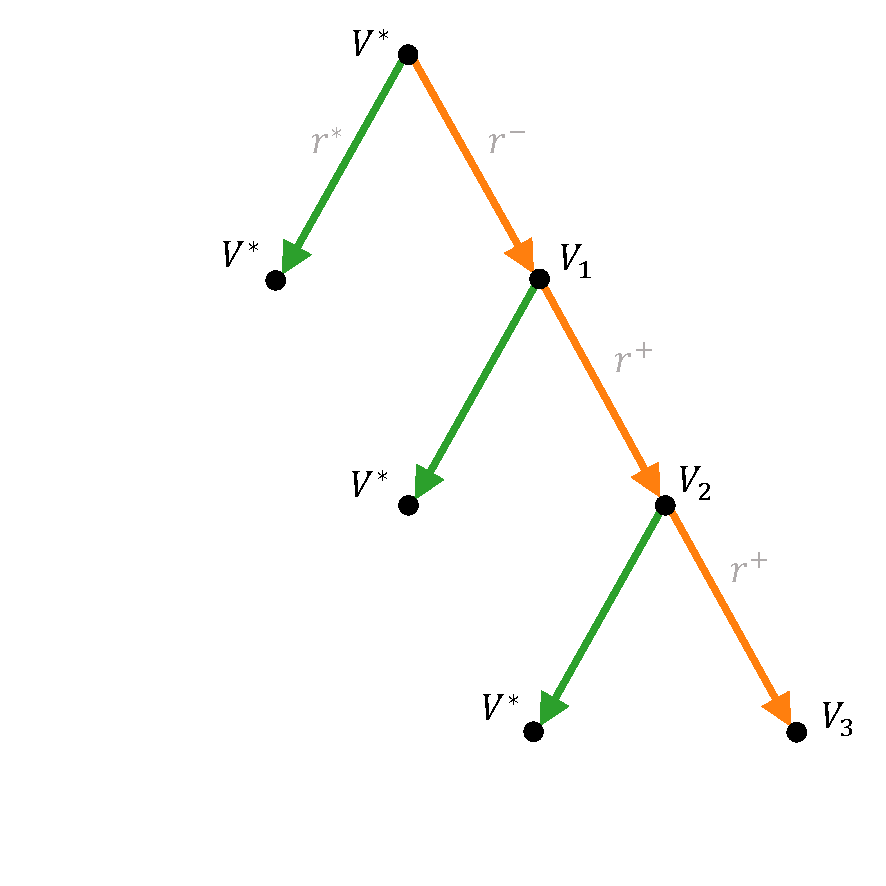
\includegraphics[trim={3.5cm 2cm 0.5cm 0.5cm}, clip, width=0.6\textwidth]{img/mdp_tree.pdf}
    \caption{Planning tree of the MDP $\cM$ of \autoref{fig:mdp}}.
    \label{fig:mdp-tree}
\end{figure}
\begin{lemma}
 Any sequence of actions in $M\setminus{a_1}$ is in $\Tau^\infty$.
\end{lemma}
\begin{proof}
Any such sequence of actions yields the sequence of rewards $r^-, r^+, \dots,r^+$. and end up in the state $s^+$ with value at least $V^*$ (obtained by further taking $a_1$ indefinitely). Thus its value $V_h$ verifies, 
\begin{align*}
    V_h &\geq \sum_{t=0}^{h-1} \gamma^t r_t + \gamma^h V^*\\
    &= r^- - r^+ + \sum_{t=0}^{h-1} \gamma^t r^+ + \gamma^h V^* \\
    &= (-\frac{\gamma}{1-\gamma} - 1)S + \frac{1-\gamma^h}{1-\gamma} (r^* + S) + \gamma^h V^*\\
    &= (-\frac{\gamma}{1-\gamma} - 1)S + \frac{1-\gamma^h}{1-\gamma} (r^* + S) + \gamma^h V^*\\
    &= V^* - S\frac{\gamma^h}{1-\gamma} \geq V^* - \frac{\gamma^h}{1-\gamma}
\end{align*}
\qed\end{proof}

We can directly conclude that $\kappa \geq \limsup{|\{a_2,\dots,a_K\}^h|^{1/h}} = K-1$.

Now, consider the nodes expanded by \autoref{alg:state-aware}. The first expansion is that of the root, which discovers $s^*$ and $s^+$. In the absence of information on these two state, the bound $V_{\max}$ is used and the first action $a_1$ gets a higher $U^a$ that any other action $a_2,\dots,a_K$ since $r^* \geq r^-$. Hence, at the second iteration, the node $a_1$ gets expanded. At this point, the self-loop of the state $s^*$ is discovered, which means that form now on the bounds verify $L_n(a_1) = V^* = U_n(a_1)$ for $n\geq2$, which means that $L_n(a_1A^*)-U_n(a_1A^*) = 0$. The nodes $a_2,\dots,a_K$ can be expanded at most once until the entire MDP is discovered and $L_n=V=U_n$ over the entire tree, which means that $\Tau_n^\infty$ is the set of optimal nodes, that is the nodes in the only optimal sequence $a_1^*$. Hence, $\kappa_\infty = 1.$ 

\section{Convergence of $(M B)^k$}
\label{sec:convergence}
\begin{figure}[H]
    \centering
    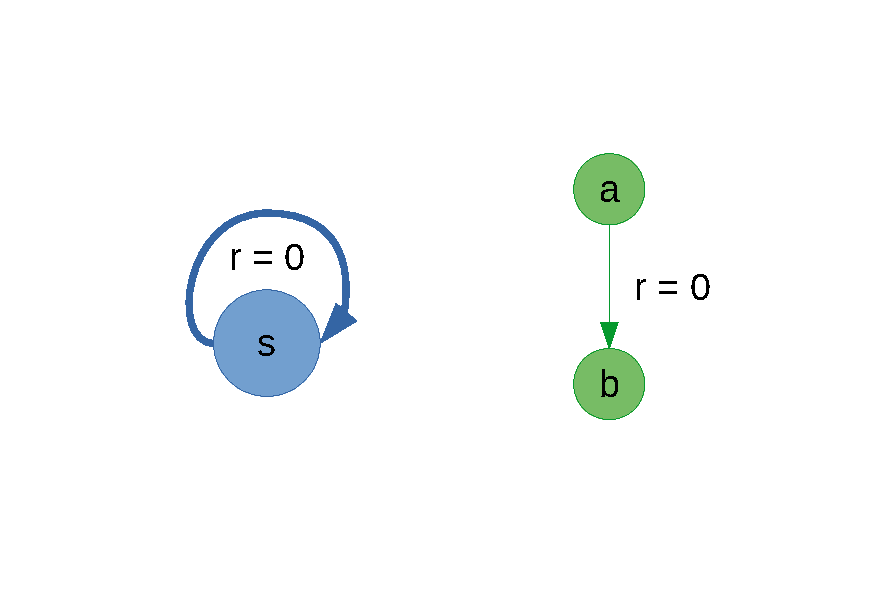
\includegraphics[trim=2cm 2cm 2cm 2cm, clip, width=0.4\textwidth]{img/simple_loop.pdf}\\
    \begin{tabular}{cccccc}
         \toprule
         Operator & $I$ & $B$ & $M B$ & $\cdots$ & $(M B)^k$ \\
         \midrule
         $U(a)$ & $V_{\max}$ & $\frac{1}{2} + \gamma V_{\max}$ & $\frac{1}{2} + \gamma V_{\max}$ && $\frac{1}{2}(1-\gamma^k)V_{\max} + \gamma^k V_{\max}$\\
         $U(b)$ & $V_{\max}$ & $V_{\max}$ & $\frac{1}{2} + \gamma V_{\max}$ && $\frac{1}{2}(1-\gamma^k)V_{\max} + \gamma^k V_{\max}$\\
         $L(a)$ & $0$ & $\frac{1}{2}$ & $\frac{1}{2}$ && $\frac{1}{2}(1-\gamma^k)V_{\max}$\\
		 $L(b)$ & $0$ & $0$ & $\frac{1}{2}$ && $\frac{1}{2}(1-\gamma^k)V_{\max}$\\
         \bottomrule
    \end{tabular}
    \caption{\textbf{Top}: a looping MDP with $|S|=|A|=1$, and the corresponding expanded tree $\Tau_1$ for a single observed transition. \textbf{Bottom}: the sequence of upper-bounds $(U_n)$ when alternating $A$ and $L$. We obtain $(U_k)$ and $(L_k)$ only go to their limit $V = \frac{1}{2}V_{\max}$ geometrically.} % TODO: r=1/2
    \label{fig:simple_loop}
\end{figure}

\section{Supplementary Experiments}
\subsection{Effect of the early stopping}

\begin{figure}[H]
    \centering
    \begin{subfigure}[b]{\textwidth}
        \centering
        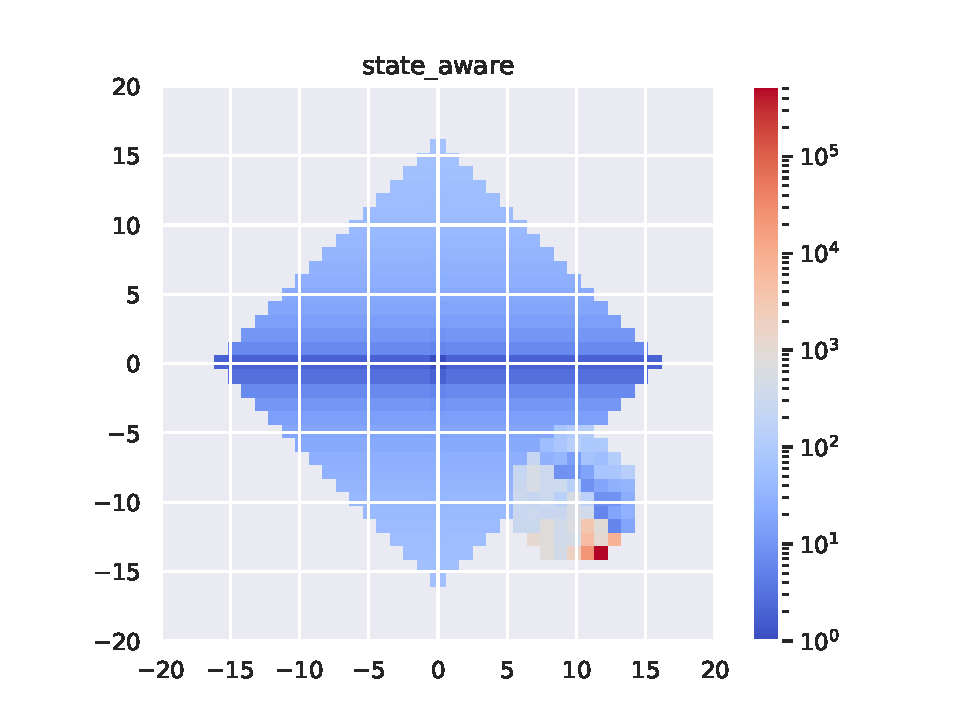
\includegraphics[width=0.49\linewidth]{img/epsilon/0/updates_state_aware.pdf}
        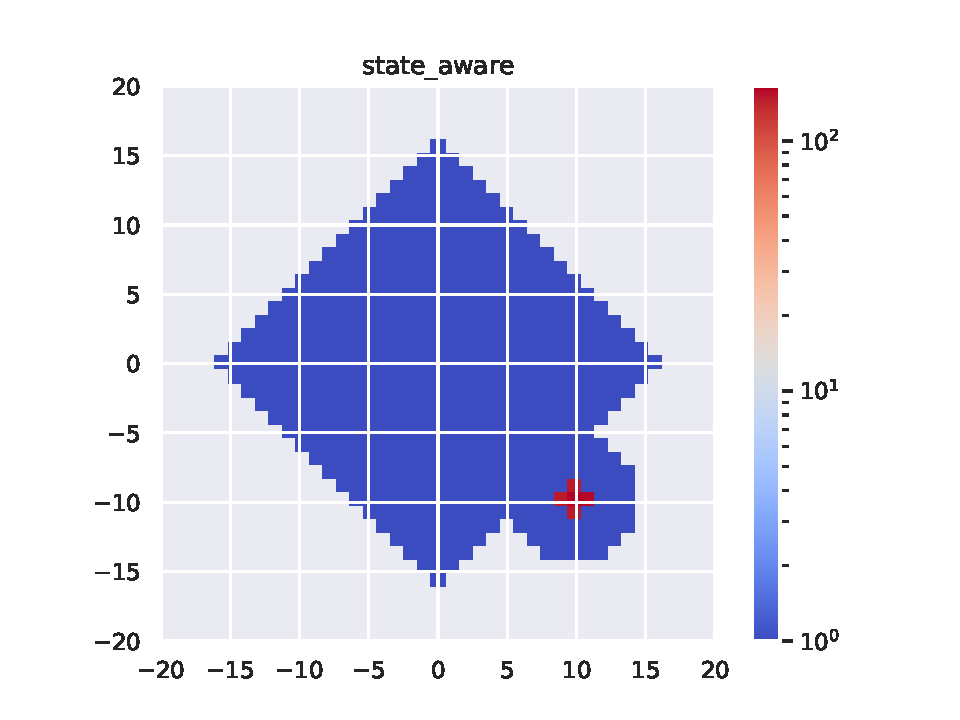
\includegraphics[width=0.49\linewidth]{img/epsilon/0/occupations_state_aware.pdf}
        \caption{$\epsilon=0$}
    \end{subfigure}
    \begin{subfigure}[b]{\textwidth}
        \centering
        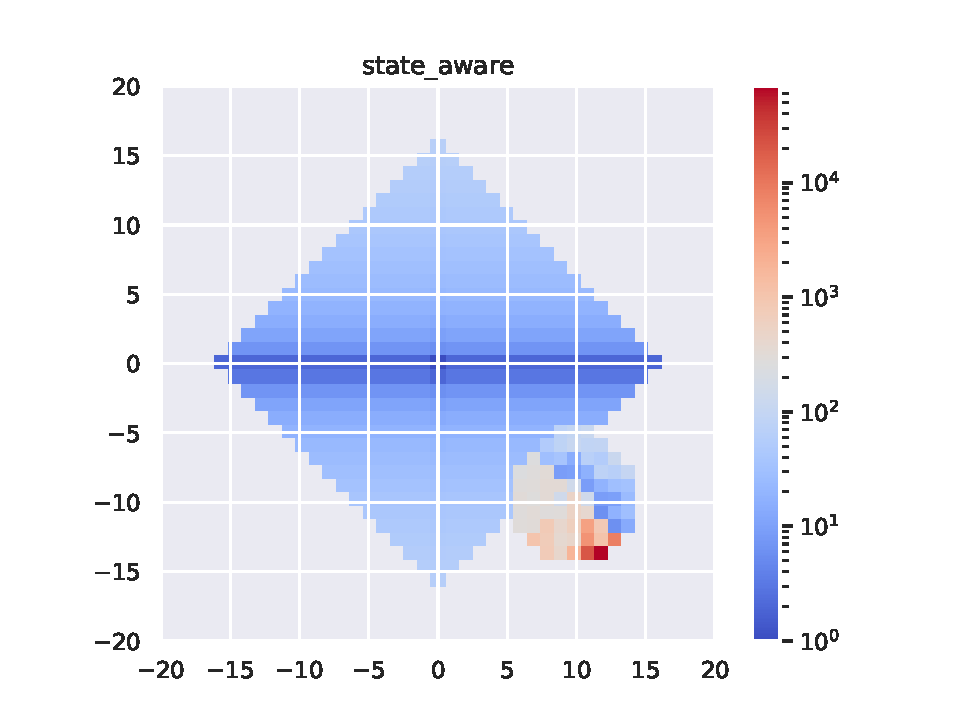
\includegraphics[width=0.49\textwidth]{img/epsilon/1e-2/updates_state_aware.pdf}
        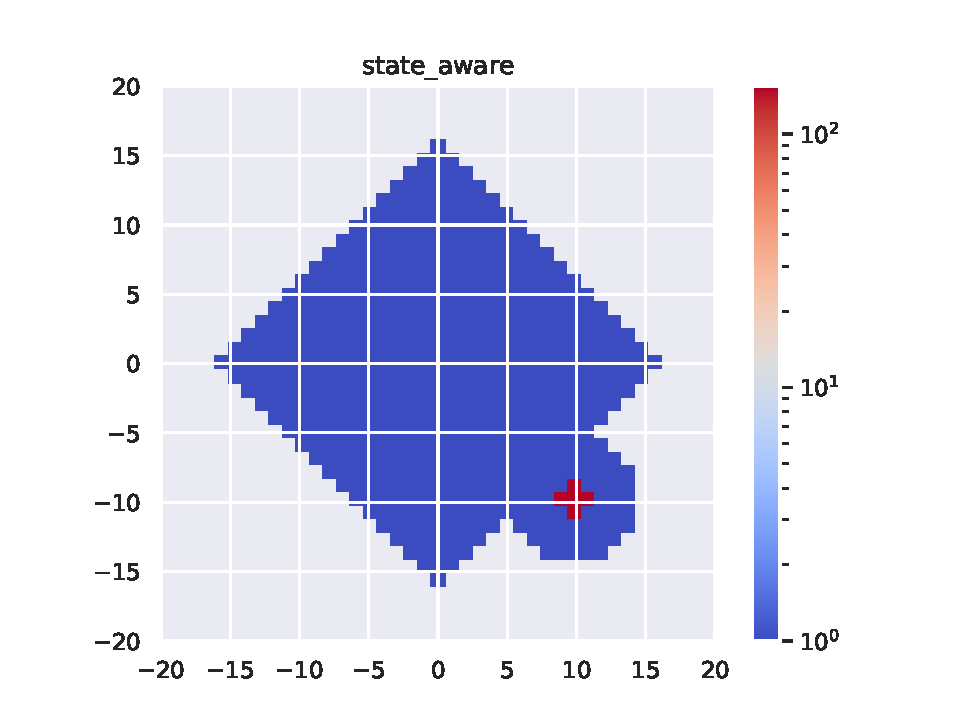
\includegraphics[width=0.49\textwidth]{img/epsilon/1e-2/occupations_state_aware.pdf}
        \caption{$\epsilon=1e-2$}
    \end{subfigure}
    \begin{subfigure}[b]{\textwidth}
        \centering
        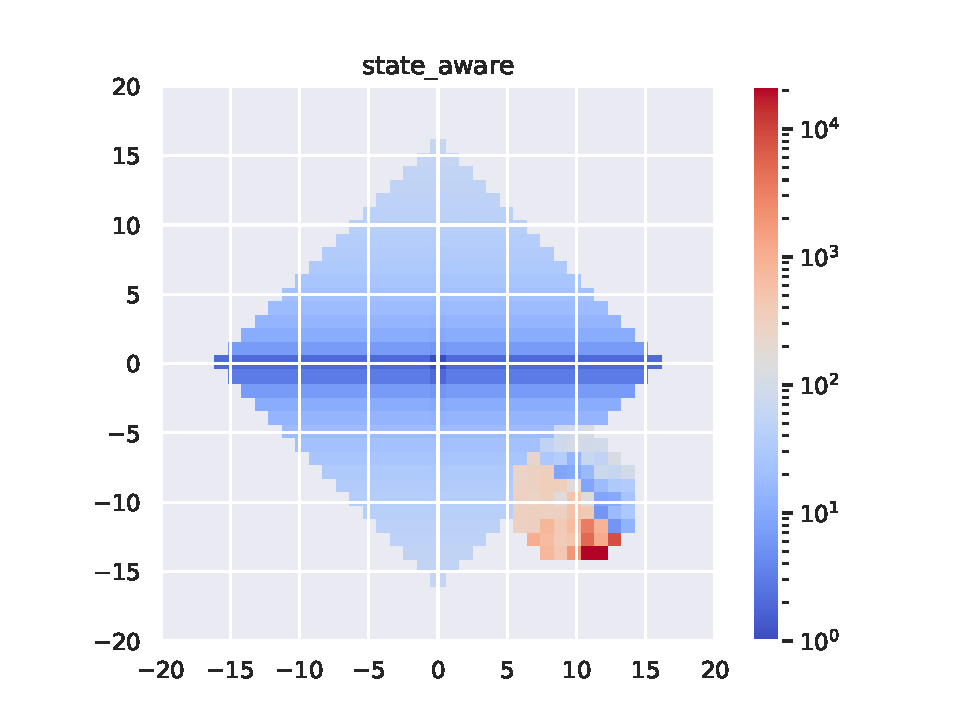
\includegraphics[width=0.49\textwidth]{img/epsilon/1e-1/updates_state_aware.pdf}
        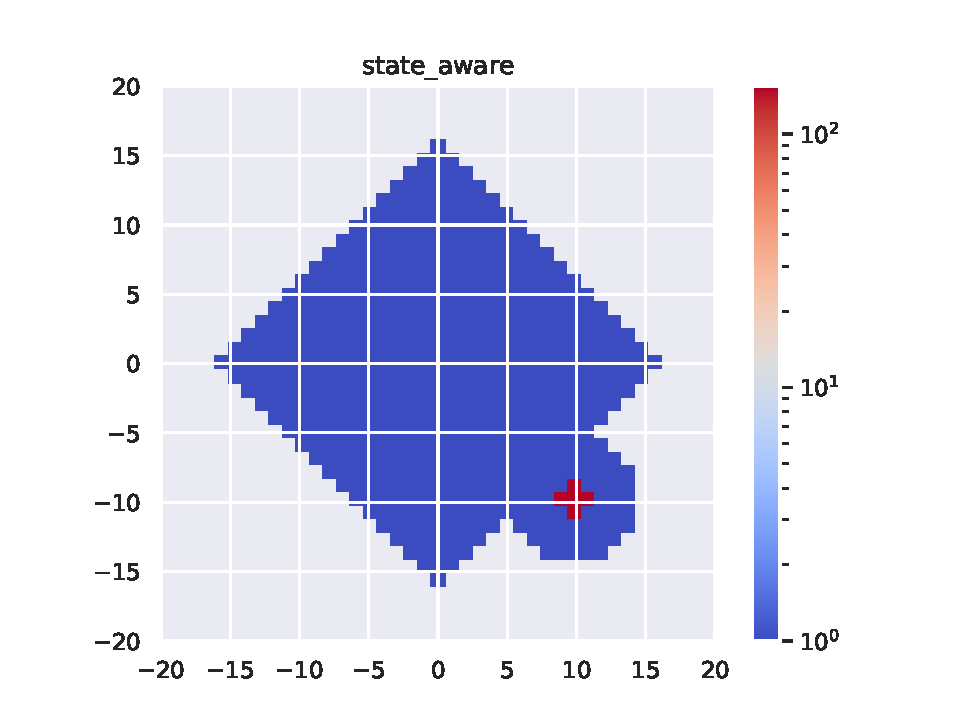
\includegraphics[width=0.49\textwidth]{img/epsilon/1e-2/occupations_state_aware.pdf}
        \caption{$\epsilon=1e-1$}
    \end{subfigure}
    \caption{Updates and occupancies for various values of $\epsilon$, for $n = 5460$, $\gamma=0.95$}
    \label{fig:epsilon_1}
\end{figure}
\begin{figure}[H]
\ContinuedFloat
    \centering
    \begin{subfigure}[b]{\textwidth}
        \centering
        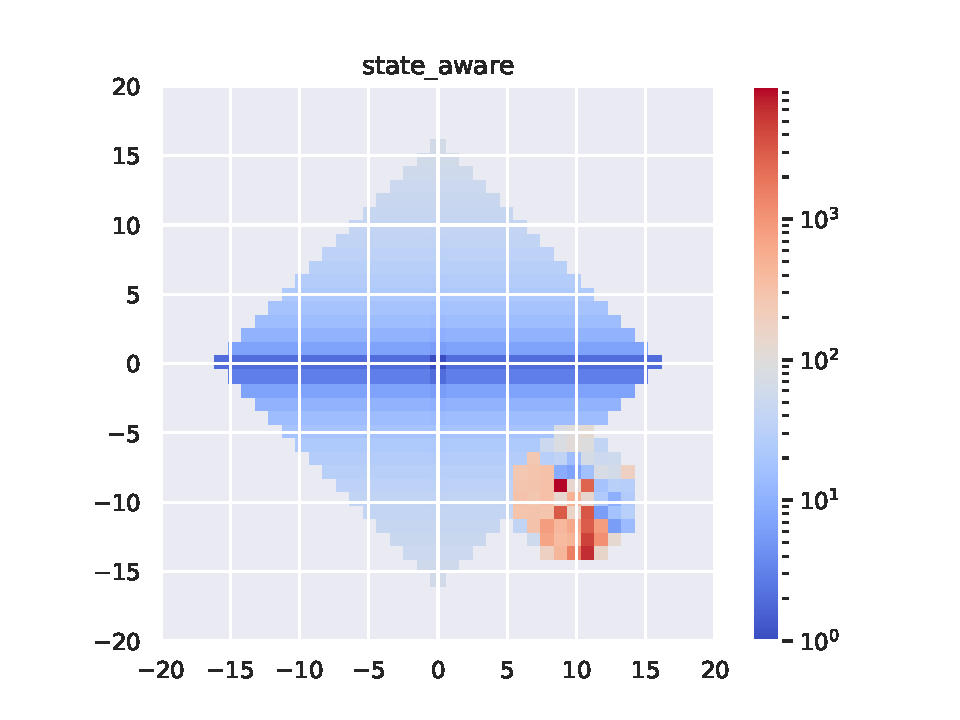
\includegraphics[width=0.49\textwidth]{img/epsilon/1e0/updates_state_aware.pdf}
        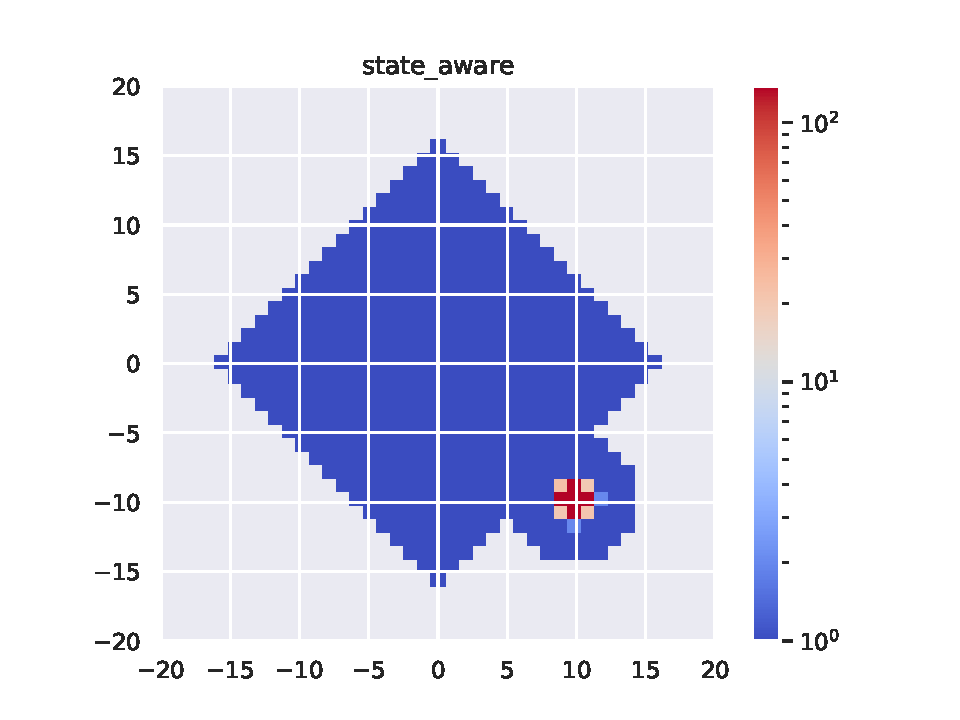
\includegraphics[width=0.49\textwidth]{img/epsilon/1e0/occupations_state_aware.pdf}
        \caption{$\epsilon=1e0$}
    \end{subfigure}
    \begin{subfigure}[b]{\textwidth}
        \centering
        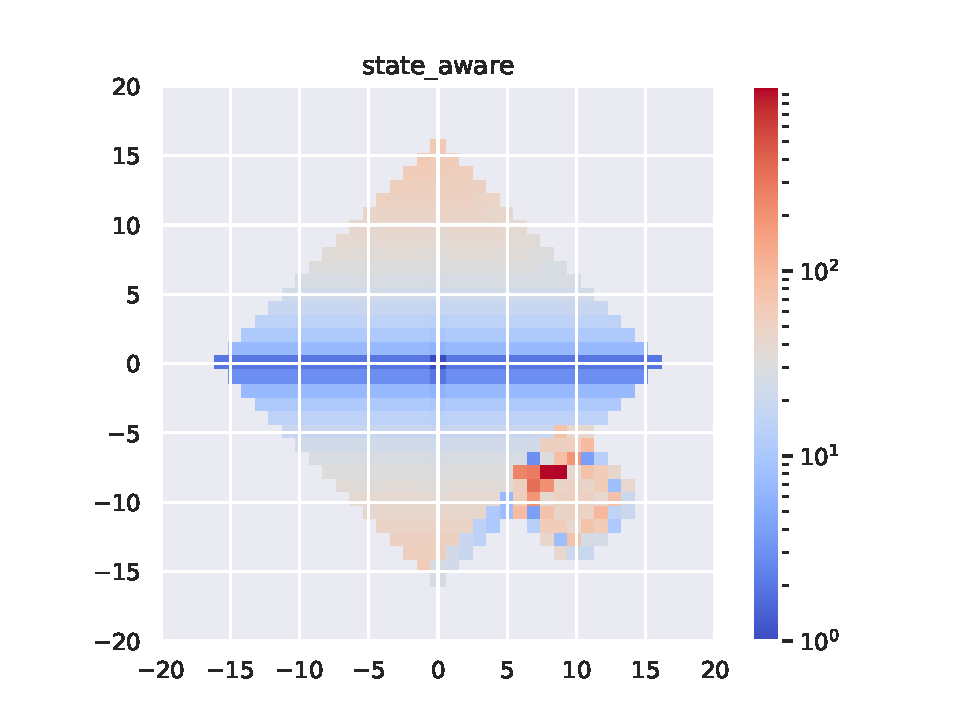
\includegraphics[width=0.49\textwidth]{img/epsilon/1e1/updates_state_aware.pdf}
        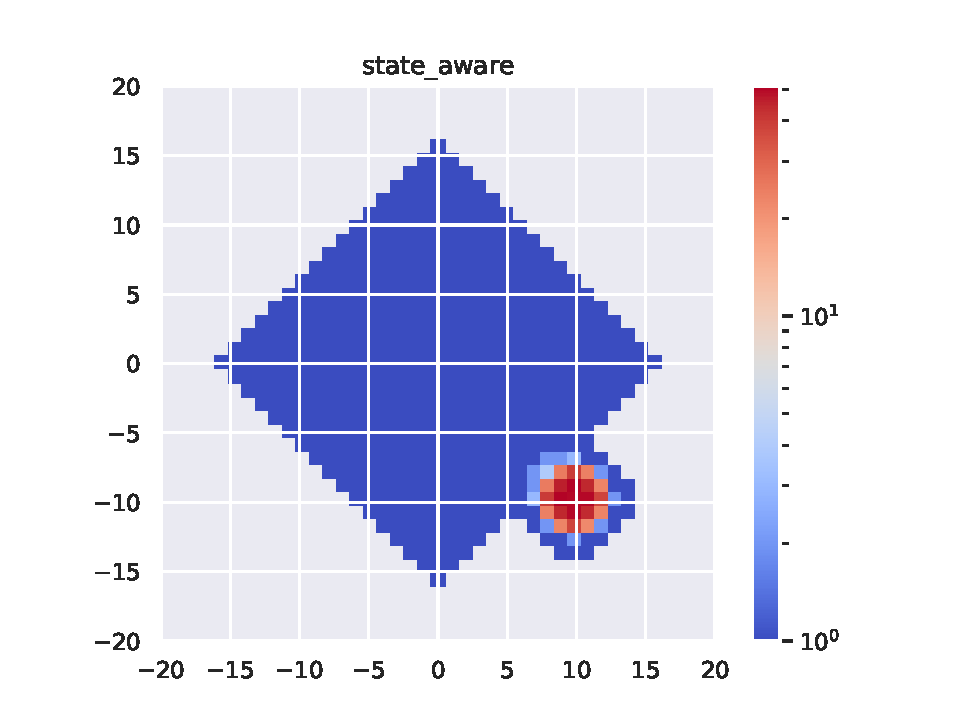
\includegraphics[width=0.49\textwidth]{img/epsilon/1e1/occupations_state_aware.pdf}
        \caption{$\epsilon=1e1$}
    \end{subfigure}
    \begin{subfigure}[b]{\textwidth}
        \centering
        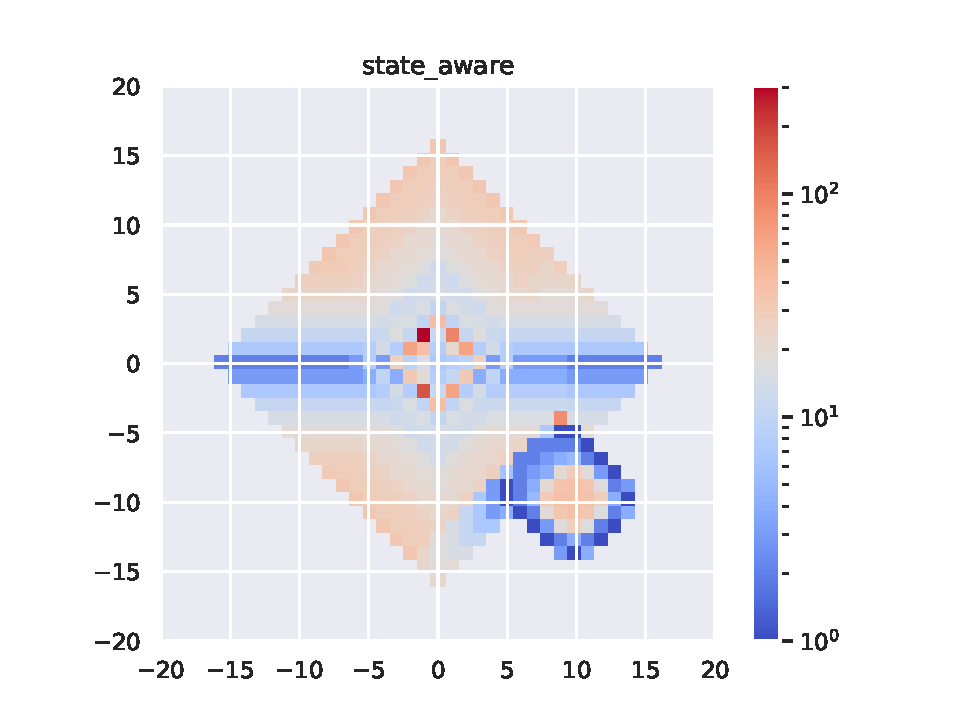
\includegraphics[width=0.49\textwidth]{img/epsilon/1e2/updates_state_aware.pdf}
        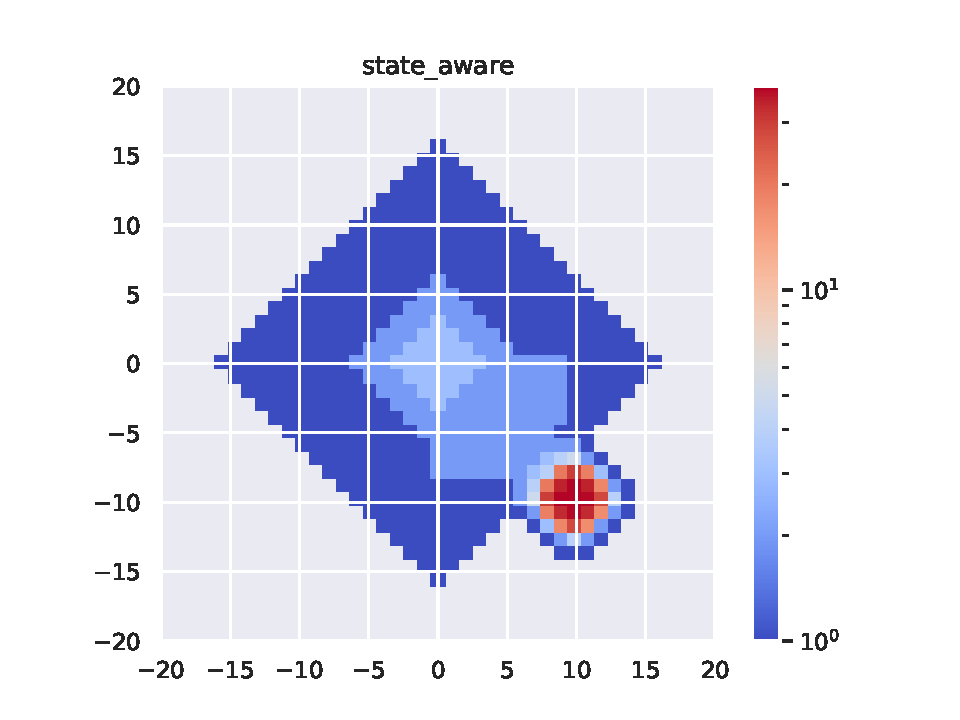
\includegraphics[width=0.49\textwidth]{img/epsilon/1e2/occupations_state_aware.pdf}
        \caption{$\epsilon=1e2 = V_{\max}$}
    \end{subfigure}
    \caption{Updates and occupancies for various values of $\epsilon$, for $n = 5460$, $\gamma=0.95$}
\end{figure}


\end{document}
